\chapter{Evaluation}
\label{sec:eval}
In this chapter, SPML will be evaluated in terms of efficiency, accuracy, latency, and privacy. The details about the experimental setup used, the data set used, and the methodology followed will be discussed in this chapter. We have implemented Differential privacy using TensorFlow privacy library \cite{11} and randomized response. The TensorFlow privacy library adds random noise from Gaussian distribution during the model's training. The measurements will help us to understand the effect of adding differential privacy on a machine learning system in terms of latency and accuracy. The measurements will be carried on two popular machine learning public datasets MNIST \cite{12} and CIFAR10 \cite{13}. We have also run measurements to study the effect of adding randomized response which is our contribution to this framework. In the end, we have evaluated our system SPML against model inversion attack to show visually how image classification can be preserved and protected by enabling privacy and security property in our system.

\section{Experimental Setup}
To evaluate our system SPML for noise, Google's open-source TensorFlow privacy library is used. The repository \cite{11} contains a Python written library and can be used to train various machine learning models with differentially private TensorFlow optimizers such as differentially private stochastic gradient descent, adam, adagrad, etc. Additionally, it also provides tools to compute the privacy that will be achieved using these optimizers. TensorFlow privacy library version 0.2.2 was used as an underlying library to conduct measurements and TensorFlow version 1.15 was used with Keras version 2.3.1. 
\subsection{Testbed}
The machine used for running experiments was Linux with 2.2 GHz Quad-Core Intel(R) Xeon(R) CPU E3-1280 v6 @ 3.90GHz with 8 cores and RAM as 64 GB. 
\subsection{Methodology}
The measurements are classified into native TensorFlow (i.e SPML) and differential privacy (DP) run (i.e SPML+privacy). Native TensorFlow run means results are achieved with the optimizers from the native TensorFlow library \cite{46} and differential privacy run results are achieved with optimizers from the TensorFlow privacy library \cite{11}. To study the effect of enabling privacy feature in SPML on an existing machine learning system, we have executed DP (SPML+privacy) runs with six different values of epsilons 0.1, 1, 2, 4, 6, and 8. These measurements will help us to understand the relationship between different values of epsilon and accuracy as well as latency.

The native TensorFlow and DP run are conducted in three different environments (1) Native environment without SGX and SCONE (2) Simulation environment with SCONE, in a docker container, and without Intel SGX (3) Hardware environment with SCONE and Intel SGX, in a docker container. Even though docker containers are involved but the performance impact of docker on SPML is out of the scope of these measurements. In SPML, we want to evaluate the effect of enabling security and privacy property on accuracy and latency. To conclude this notion, each dataset will have a total of six experimental runs i.e native TensorFlow and DP run with three environments.

We will evaluate SPML for both of the phases of the machine learning system which are training and inference phase. Each phase will have six experiments as discussed above. For each phase, the final accuracy and latency score is an average of 10 iterations with 5 epochs for each epsilon value. In the next sections, the dataset and their evaluation are discussed.
\section{MNIST}
\label{sec:evalMnist}
The MNIST is a handwritten digits database \cite{12}. The original set has 60,000 training example but for this experiment, this dataset is reduced to use 10,000 examples for the training phase. These images are greyscaled and centered in a 28x28 image. For the inference phase, a dataset of 10,000 images from the original set is extracted and used for evaluating the trained model. Each of the pictures can be categorized as one of the digits from 0 to 9. For training the model, a convolutional neural network is used. It has two layers of convolution, each of this convolution layer follows a max-pooling layer. After these layers, a flatten layer is added followed by two dense layers. Both the Convolutional layers and one of the dense layer have rectified linear unit (ReLU ) activation function. These layers are connected using TensorFlow Python APIs. In the next subsections, training and inference results are discussed. 
\subsection{Training phase}
This subsection is organized into three parts as native mode, SCONE simulation mode, and SCONE hardware mode. In other words, we can say native mode means only enabling privacy property, SCONE hardware mode means enabling both privacy and security property. SCONE simulation mode gave us an idea about the overhead of running SPML in a SCONE runtime environment. For each mode, we will discuss the impact on accuracy and latency.

\subsubsection{Native Mode}
\begin{figure}
     \begin{subfigure}{0.5\textwidth}
         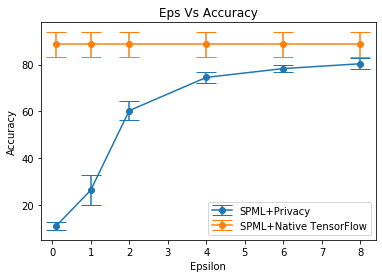
\includegraphics[width=\textwidth]{images/Training/MnistNativeAccuracy.png}
         \caption{Accuracy}
         \label{fig:nativeMnistAccuracyTraining}
     \end{subfigure}
     \begin{subfigure}{0.5\textwidth}
         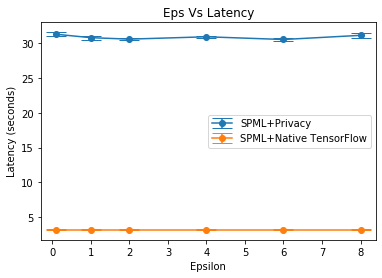
\includegraphics[width=\textwidth]{images/Training/MnistNativeLatency.png}
         \caption{Latency}
         \label{fig:nativeMnistLatencyTraining}
     \end{subfigure}
        \caption{MNIST Dataset - Training - Native mode without Intel SGX and SCONE}
     \begin{subfigure}{0.5\textwidth}
         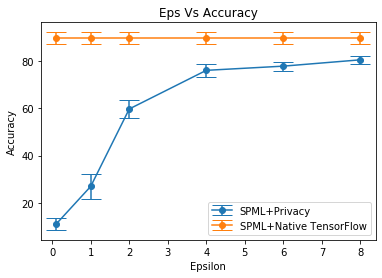
\includegraphics[width=\textwidth]{images/Training/MnistSimAccuracy.png}
         \caption{Accuracy}
         \label{fig:simMnistAccuracyTraining}
     \end{subfigure}
     \begin{subfigure}{0.5\textwidth}
         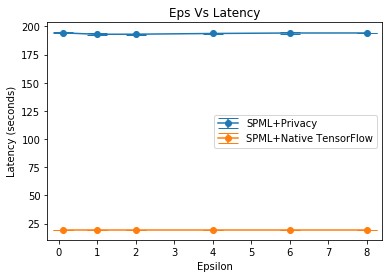
\includegraphics[width=\textwidth]{images/Training/MnistSimLatency.png}
         \caption{Latency}
         \label{fig:simMnistLatencyTraining}
     \end{subfigure}
        \caption{MNIST Dataset - Training - Simulation mode without Intel SGX and with SCONE}
     \begin{subfigure}{0.5\textwidth}
         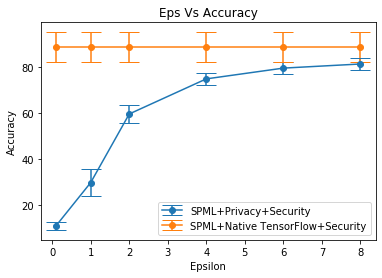
\includegraphics[width=\textwidth]{images/Training/MnistHWAccuracy.png}
         \caption{Accuracy}
         \label{fig:hwMnistAccuracyTraining}
     \end{subfigure}
     \begin{subfigure}{0.5\textwidth}
         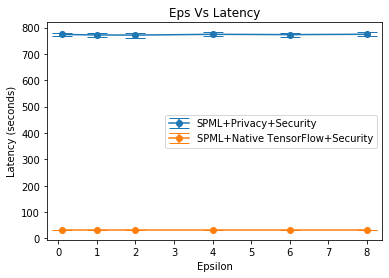
\includegraphics[width=\textwidth]{images/Training/MnistHWLatency.png}
         \caption{Latency}
         \label{fig:hwMnistLatencyTraining}
     \end{subfigure}
        \caption{MNIST Dataset - Training - Hardware mode with Intel SGX and SCONE}
\end{figure}
\begin{figure}
     \begin{subfigure}{0.5\textwidth}
         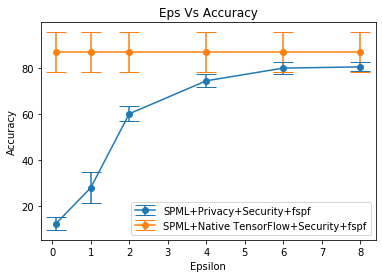
\includegraphics[width=\textwidth]{images/Training/MnistHWFSPFAccuracy.png}
         \caption{Accuracy}
         \label{fig:fspfMnistAccuracyTraining}
     \end{subfigure}
     \begin{subfigure}{0.5\textwidth}
         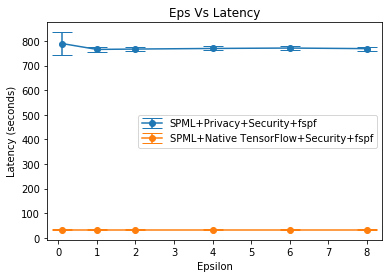
\includegraphics[width=\textwidth]{images/Training/MnistHWFSPFLatency.png}
         \caption{Latency}
         \label{fig:fspfMnistLatencyTraining}
     \end{subfigure}
        \caption{MNIST Dataset - Training - Hardware mode + Fspf with Intel SGX and SCONE}
\end{figure}
\textbf{\textit{Accuracy: }}The accuracy here means the rate at which we predict or classify the correct data out of the whole set. Figure ~\ref{fig:nativeMnistAccuracyTraining} shows the native mode measurements of the MNIST dataset for accuracy. The SPML+native TensorFlow run achieved accuracy of 88\%. SPML+Privacy runs shows an increasing trend from epsilon value 0.1 to 8. With epsilon value 0.1, only accuracy of 11\% is achieved. The accuracy kept on increasing as epsilon value is increased and accuracy of 80\% is achieved at epsilon value 8. This is because as we increase the epsilon value the noise level decreases, hence accuracy value should increase. This notion is clearly shown in Figure ~\ref{fig:nativeMnistAccuracyTraining}. Hence, we can say that at smaller epsilon values we protect strongly, but this will lead to some degradation in accuracy. This is always a trade-off to decide at what level we need protection and accuracy.
\newline
\newline
\textbf{\textit{Latency: }}The Figure ~\ref{fig:nativeMnistLatencyTraining} shows the native mode measurements of the MNIST dataset for latency. The SPML+native TensorFlow run shows the latency of 3 seconds. All the SPML+Privacy runs for different values of epsilons show almost the same latency value of 30 seconds. This means latency doesn't change much with different epsilon values. The SPML+Privacy runs have almost 10$\times$ latency as compare to SPML+native TensorFlow runs. Hence, we can say that this is the approximation cost in terms of latency for adding privacy property into our system SPML. Next, we will look into the accuracy and latency values for running SPML in SCONE runtime environment.


\subsubsection{SCONE simulation mode}
\textbf{\textit{Accuracy: }} In SCONE simulation mode, the accuracy trend as explained above remains the same. As in the previous measure of SPML in native mode (i.e without Intel SGX and SCONE), we have seen that accuracy increases as epsilon value increases. Figure ~\ref{fig:simMnistAccuracyTraining} shows the epsilon value of 0.1 achieves an accuracy of 10\% and the epsilon value of 8 achieves an accuracy of 80\%. The accuracy trend in SCONE simulation mode for SPML+Privacy and SPML+native TensorFlow run is almost the same as the native (i.e without Intel SGX and SCONE) mode run. Hence, we can say that simulation mode has very little or no effect on accuracy.
\begin{table}[h!]
  \begin{center}
    \caption{MNIST Latency Comparison - Training }
    \label{tab:mnistLatencyTraining}
    \begin{tabular}{|c|c|c|}
      \hline
      \textbf{} & \textbf{SPML +} & \textbf{SPML +} \\
      \textbf{} & \textbf{native TensorFlow} & \textbf{privacy} \\
      \textbf{} & \textbf{(seconds)} & \textbf{(seconds)} \\
      \hline
      \textbf{Native mode} & 3        &   30\\
      \hline
      \textbf{SCONE simulation mode} &  19       &     195\\
      \hline    
      \textbf{SCONE hardware mode} &    32     &      775\\
      \hline
    \end{tabular}
   \end{center}
\end{table}
\newline
\newline
\textbf{\textit{Latency: }}The latency of SPML as shown in ~\ref{fig:simMnistLatencyTraining} remains almost constant for all epsilon value around 195 seconds and the SPML+native TensorFlow run has a latency of around 19 seconds. The table ~\ref{tab:mnistLatencyTraining} shows quick comparison of latency for all modes. The latency for simulation mode is 6$\times$ times higher as compared to the native(i.e without Intel SGX and SCONE) mode for SPML+Privacy and SPML+native TensorFlow run. This means this is the cost of enabling privacy property in SPML in SCONE simulation mode. In the next experiment, we want to evaluate security property in SCONE hardware mode.

\subsubsection{SCONE hardware mode}
The hardware mode means running SPML with Intel SGX and SCONE environment. SCONE FSPF \cite{77} is needed to transparently encrypt/decrypt the data, code, and model. SCONE FSPF perform cryptography related operation using Intel-CPU-specific hardware instructions. In this section, we have evaluated our system SPML for both choices, if we enable file system shield (i.e FSPF) and if we don't enable this shield (i.e without FSPF). It should not make any difference if we run SPML with FSPF and without FSPF as measurement should be ideally the same for both of these options. We will be discussing results for both the choices in next paragraph.
\newline
\newline
\textbf{\textit{Accuracy: }} In SCONE hardware mode also, the accuracy trend remains the same. As seen in the previous measurement of the accuracy of SPML in native and simulation mode, we have seen that accuracy increases as epsilon value increases. Figure ~\ref{fig:hwMnistAccuracyTraining}, ~\ref{fig:fspfMnistAccuracyTraining} shows that the accuracy trends increase from 10 to 80 \% for 0.1 and 8 epsilon value respectively without and with FSPF. Hence this shows that the accuracy trend in SCONE hardware mode(with FSPF and without FSPF) for SPML+privacy and SPML+native TensorFlow run is almost the same as native or simulation mode run. Hence, we can say that hardware mode has very little or no effect on the accuracy of SPML like SCONE simulation mode.
\newline 
\newline
\textbf{\textit{Latency: }}The latency as shown in Figure ~\ref{fig:hwMnistLatencyTraining}, ~\ref{fig:fspfMnistLatencyTraining} remain almost constant for all epsilon value around 775 seconds with SPML+privacy run without and with FSPF. On the other hand, the SPML+native TensorFlow run has a latency of around 38 seconds. Hardware mode means security is enabled by default. So we can say the SPML system is SPML + security. As shown in Table ~\ref{tab:mnistLatencyTraining}, SPML+security+privacy has 24$\times$ latency as compared to SPML+security without privacy. The latency for hardware mode is 4$\times$, 25$\times$ times higher as compared to simulation, and the native mode for SPML+security+privacy respectively. The SPML+security without privacy run has latency almost 1.5$\times$, 10.5$\times$ as compare to the SPML without privacy run in simulation and native mode respectively.

For hardware mode, the training accuracy and latency trends with FSPF and without FSPF are almost the same. It means transparent encryption/decryption by SCONE for code, data and model are not adding any overhead in terms of latency and accuracy. We have run FSPF mode only for the MNIST dataset to conclude this notion.

It is seen that hardware mode, which is enabling security property in our system SPML, has very high latency. The reason for this is the small EPC size, where code, data, and model are executed. The EPC size is 90MB and the classification process usually takes 330MB of main memory and the process is independent of training size (i.e number of images) \cite{81}. Therefore, paging is required as EPC memory is exceeded during this process, which is achieved using page swap to non-encrypted main memory. To protect the data again after swapping, the encryption process needs to be repeated. Hence this leads to the poor performance of read and writes, and degrades overall performance in terms of latency.

However, on the other hand, privacy, confidentiality, and integrity are also added on code, data, and model. Hence we can say that this is the cost in terms of latency one needs to take for training the models. The good thing is that in practice, we can perform training over the weekend or as nightly run to save efforts and time for developers. Hence this extra latency can be avoided and dealt with if planned well in advance. However, the inference is used more frequently to predict or classify, so it should have latency within reasonable limits so that our SPML system can be used in the normal office working hours. In the next section, we want to evaluate the SPML system for the inference phase.
\subsection{Inference phase}
This subsection is organized into two parts as accuracy and latency and all three modes are discussed.
\begin{figure}
     \begin{subfigure}{0.5\textwidth}
         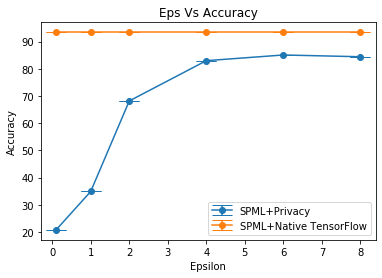
\includegraphics[width=\textwidth]{images/Inference/MnistNativeAccuracyInference.png}
         \caption{Accuracy}
         \label{fig:nativeMnistAccuracyInference}
     \end{subfigure}
     \begin{subfigure}{0.5\textwidth}
         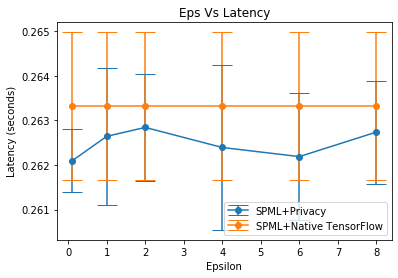
\includegraphics[width=\textwidth]{images/Inference/MnistNativeLatencyInference.png}
         \caption{Latency}
         \label{fig:nativeMnistLatencyInference}
     \end{subfigure}
        \caption{MNIST Dataset - Inference - Native mode without Intel SGX and SCONE}
     \begin{subfigure}{0.5\textwidth}
         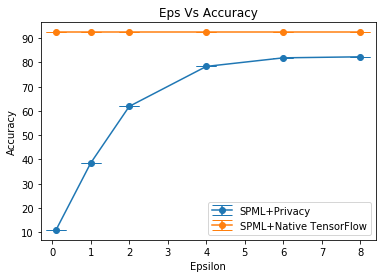
\includegraphics[width=\textwidth]{images/Inference/MnistSimAccuracyInference.png}
         \caption{Accuracy}
         \label{fig:simMnistAccuracyInference}
     \end{subfigure}
     \begin{subfigure}{0.5\textwidth}
         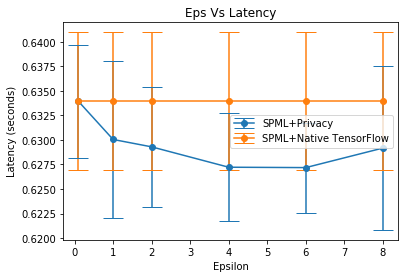
\includegraphics[width=\textwidth]{images/Inference/MnistSimLatencyInference.png}
         \caption{Latency}
         \label{fig:simMnistLatencyInference}
     \end{subfigure}
        \caption{MNIST Dataset - Inference - Simulation mode without Intel SGX and with SCONE}
     \begin{subfigure}{0.5\textwidth}
         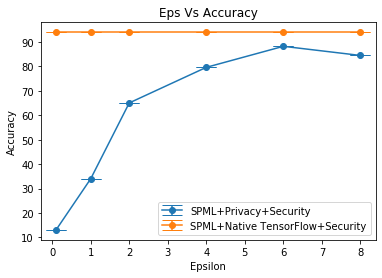
\includegraphics[width=\textwidth]{images/Inference/MnistHwAccuracyInference.png}
         \caption{Accuracy}
         \label{fig:hwMnistAccuracyInference}
     \end{subfigure}
     \begin{subfigure}{0.5\textwidth}
         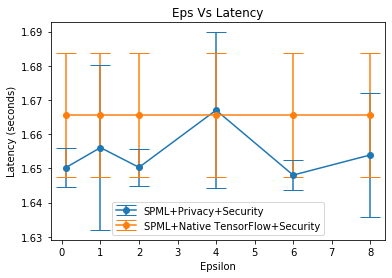
\includegraphics[width=\textwidth]{images/Inference/MnistHwLatencyInference.png}
         \caption{Latency}
         \label{fig:hwMnistLatencyInference}
     \end{subfigure}
        \caption{MNIST Dataset - Inference - Hardware mode with Intel SGX and SCONE}
\end{figure}
\begin{figure}
     \begin{subfigure}{0.5\textwidth}
         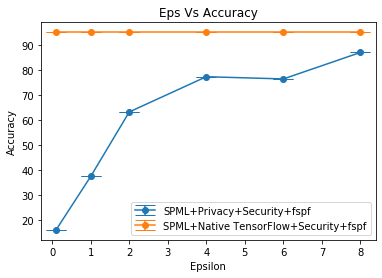
\includegraphics[width=\textwidth]{images/Inference/MnistFSPFAccuracyInference.png}
         \caption{Accuracy}
         \label{fig:fspfMnistAccuracyInference}
     \end{subfigure}
     \begin{subfigure}{0.5\textwidth}
         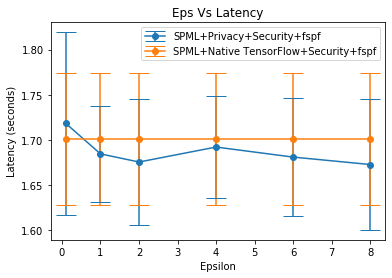
\includegraphics[width=\textwidth]{images/Inference/MnistFSPFLatencyInference.png}
         \caption{Latency}
         \label{fig:fspfMnistLatencyInference}
     \end{subfigure}
        \caption{MNIST Dataset - Inference - Hardware mode + Fspf with Intel SGX and SCONE}
\end{figure}
\newline
\newline
\textbf{\textit{Accuracy: }}The inference figures of accuracy for native, simulation, and hardware mode without and with FSPF are shown in Figure ~\ref{fig:nativeMnistAccuracyInference}, ~\ref{fig:simMnistAccuracyInference}, ~\ref{fig:hwMnistAccuracyInference}, ~\ref{fig:fspfMnistAccuracyInference}  respectively. Accuracy depends upon the model that is being trained and used for doing inference. If the model trained and saved have good accuracy then inferences have good accuracy. Inference accuracy in all three modes is almost the same for example the SPML+native TensorFlow model is giving an accuracy of around 94\% and the hardware is giving an accuracy of around 93.98\%. Hence accuracy in the inference phase also remains nearly comparable to the native environment and the accuracy trend remains the same which is accuracy increases as epsilon value increases.
\newline
\newline
\textbf{\textit{Latency: }}The inference figures of latency for native, simulation, and hardware mode without and with FSPF are shown in Figure ~\ref{fig:nativeMnistLatencyInference}, ~\ref{fig:simMnistLatencyInference}, ~\ref{fig:hwMnistLatencyInference}, ~\ref{fig:fspfMnistLatencyInference} respectively. The figures show that the time taken for inference is almost the same for differentially private as well as native TensorFlow algorithms. The inference has less effect in terms of whether the model is trained with differential privacy or native TensorFlow. The time taken for inference is also very less as compared to the time taken in training the models. For example, in hardware mode (SPML+Privacy+Security) inference takes around 1.66 seconds while training takes around 775 seconds and there is a huge difference between the time taken for training and inference. \newline
\begin{table}[h!]
  \begin{center}
    \caption{MNIST Latency Comparison - Inference }
    \label{tab:mnistLatencyInference}
    \begin{tabular}{|c|c|c|}
      \hline
      \textbf{} & \textbf{SPML +} & \textbf{SPML +} \\
      \textbf{} & \textbf{native TensorFlow} & \textbf{privacy} \\
      \textbf{} & \textbf{(seconds)} & \textbf{(seconds)} \\
      \hline
      \textbf{Native mode} & .26        &   .26\\
      \hline
      \textbf{SCONE simulation mode} &  .63       &     .63\\
      \hline    
      \textbf{SCONE hardware mode} &    1.66     &      1.66\\
      \hline
    \end{tabular}
   \end{center}
\end{table}
As shown in table ~\ref{tab:mnistLatencyInference}, the native (i.e without Intel SGX and SCONE) mode is completed within 0.26 seconds and hardware (i.e with Intel SGX and SCONE) takes around 1.66 seconds. Hardware mode has, 6.3$\times$ latency as compared to native and 2.63$\times$ than simulation mode respectively. The simulation mode has 2.4$\times$ latency as compared to native mode for both SPML+native Tensorflow and SPML+Privacy runs. Hence, inference doesn't increase a lot of computational overhead in terms of latency for simulation or hardware mode. There is some overhead but it is within acceptable limits to use it in practice. Next, we have evaluated the Cifar10 dataset results to study and understand if we can draw the same conclusion with this dataset also.

\section{Cifar10}
\label{sec:evalCifar10}
The Cifar10 database\cite{13} has 60000 32x32 training images. These images belong to 10 classes such as airplanes, automobiles, birds, etc. For training the model convolutional neural network is used. It has three layers of convolution, first two convolution layer follows a max pooling layer. After these layers, a flatten layer is added followed by two dense layers. Both the convolutional layers and one of the dense layer have rectified linear unit (ReLU ) activation function. These all layers are connected together using TensorFlow Python APIs. In the next subsections, training and inference results are discussed.
\subsection{Training phase}
\textbf{\textit{Accuracy: }} The notion of accuracy which we saw in the last section is same for this dataset also. The accuracy trend increases with epsilon value in all three modes. As can be seen in Figure ~\ref{fig:nativeCifar10AccuracyTraining}, ~\ref{fig:simCifar10AccuracyTraining}, ~\ref{fig:hwCifar10AccuracyTraining} for all modes, accuracy starts from around 10\% and goes upto 15\% at 0.1 and 8 epsilon value respectively. Hence it is true for this dataset also that accuracy is effected very little by the environment or the mode.
\begin{figure}
     \begin{subfigure}{0.5\textwidth}
         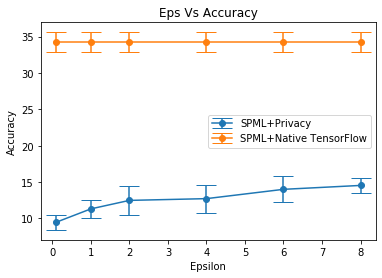
\includegraphics[width=\textwidth]{images/Training/Cifar10NativeAccuracy.png}
         \caption{Accuracy}
         \label{fig:nativeCifar10AccuracyTraining}
     \end{subfigure}
     \begin{subfigure}{0.5\textwidth}
         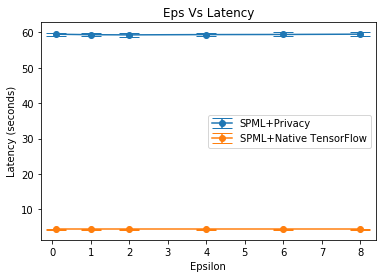
\includegraphics[width=\textwidth]{images/Training/Cifar10lNativeLatency.png}
         \caption{Latency}
         \label{fig:nativeCifar10LatencyTraining}
     \end{subfigure}
        \caption{Cifar10 Dataset - Training - Native mode without Intel SGX and SCONE}
     \begin{subfigure}{0.5\textwidth}
         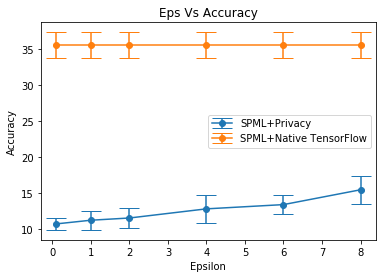
\includegraphics[width=\textwidth]{images/Training/Cifar10SimAccuracy.png}
         \caption{Accuracy}
         \label{fig:simCifar10AccuracyTraining}
     \end{subfigure}
     \begin{subfigure}{0.5\textwidth}
         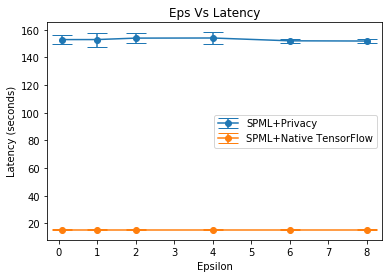
\includegraphics[width=\textwidth]{images/Training/Cifar10SimLatency.png}
         \caption{Latency}
         \label{fig:simCifar10LatencyTraining}
     \end{subfigure}
        \caption{Cifar10 Dataset - Training - Simulation mode without Intel SGX and with SCONE}
     \begin{subfigure}{0.5\textwidth}
         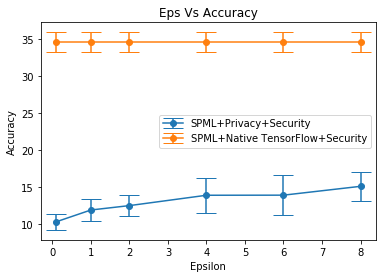
\includegraphics[width=\textwidth]{images/Training/Cifar10HWAccuracy.png}
         \caption{Accuracy}
         \label{fig:hwCifar10AccuracyTraining}
     \end{subfigure}
     \begin{subfigure}{0.5\textwidth}
         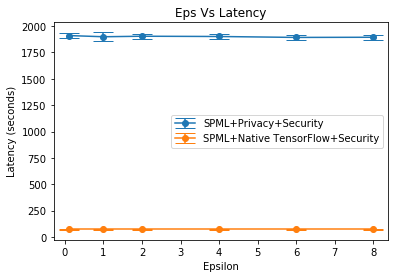
\includegraphics[width=\textwidth]{images/Training/Cifar10HWLatency.png}
         \caption{Latency}
         \label{fig:hwCifar10LatencyTraining}
     \end{subfigure}
        \caption{Cifar10 Dataset - Training - Hardware mode with Intel SGX and SCONE}
\end{figure}
\newline
\newline
\textbf{\textit{Latency: }}The latency graphs for this dataset are shown in Figure ~\ref{fig:nativeCifar10LatencyTraining}, ~\ref{fig:simCifar10LatencyTraining}, ~\ref{fig:hwCifar10LatencyTraining}. Latency doesn't increase or decrease much with the epsilon values. However, the latency of native vs simulation vs hardware mode has huge gap among themselves. The hardware mode (SPML+security+privacy) latency for Cifar10 dataset is 2030 seconds which is almost 13.35$\times$, 34.4$\times$ as compared to simulation(152 seconds) and native (59 seconds) mode latency for DP(SPML+privacy) run respectively. For native TensorFlow run(SPML+native TensorFlow), the hardware mode (SPML+security) latency is 5$\times$, 18.75$\times$ as compared to simulation and native mode latency. Hence, it can be concluded that hardware mode adds some overhead for latency for our system SPML, but at the same time we are getting a trained privacy preserving secure model. As discussed above, these latency can be tolerated and training can be planned using overnight or over weekends to save time. We evaluated inference results also to see if these can be used in practise like MNIST dataset.

\subsection{Inference phase}
\textbf{\textit{Accuracy: }} The figures ~\ref{fig:nativeCifar10AccuracyInference}, ~\ref{fig:simCifar10AccuracyInference}, ~\ref{fig:hwCifar10AccuracyInference} shows the accuracy trend for the Cifar10 dataset for inference for all the three modes. The native TensorFlow accuracy for all the modes remains the same between 9-10 \%. Since we used only 3000 images for training the model, hence for all epsilon values the same kind of inference trend is shown. With these result, it can be concluded that accuracy of native vs simulation vs hardware mode remains almost same and inference accuracy like training is not much affected by the environment.
\begin{figure}
     \begin{subfigure}{0.5\textwidth}
         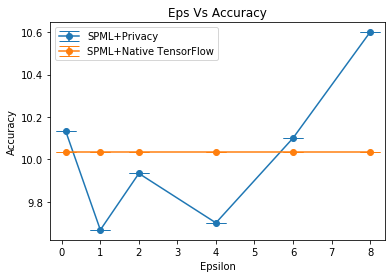
\includegraphics[width=\textwidth]{images/Inference/Cifar10NativeAccuracyInference.png}
         \caption{Accuracy}
         \label{fig:nativeCifar10AccuracyInference}
     \end{subfigure}
     \begin{subfigure}{0.5\textwidth}
         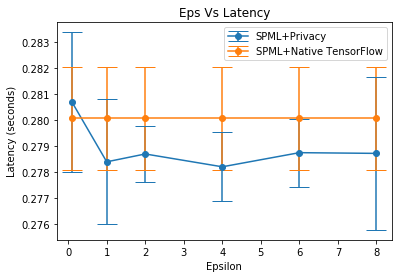
\includegraphics[width=\textwidth]{images/Inference/Cifar10NativeLatencyInference.png}
         \caption{Latency}
         \label{fig:nativeCifar10LatencyInference}
     \end{subfigure}
        \caption{Cifar10 Dataset - Inference - Native mode without Intel SGX and SCONE}
     \begin{subfigure}{0.5\textwidth}
         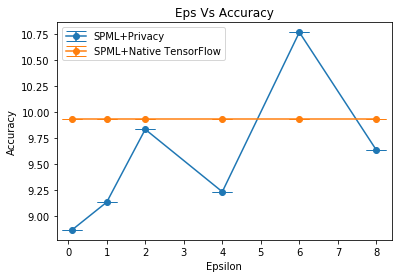
\includegraphics[width=\textwidth]{images/Inference/Cifar10SimAccuracyInference.png}
         \caption{Accuracy}
         \label{fig:simCifar10AccuracyInference}
     \end{subfigure}
     \begin{subfigure}{0.5\textwidth}
         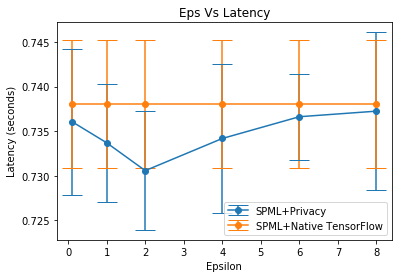
\includegraphics[width=\textwidth]{images/Inference/Cifar10SimLatencyInference.png}
         \caption{Latency}
         \label{fig:simCifar10LatencyInference}
     \end{subfigure}
        \caption{Cifar10 Dataset - Inference - Simulation mode without Intel SGX and with SCONE}
     \begin{subfigure}{0.5\textwidth}
         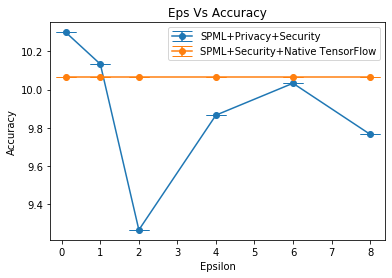
\includegraphics[width=\textwidth]{images/Inference/Cifar10HwAccuracyInference.png}
         \caption{Accuracy}
         \label{fig:hwCifar10AccuracyInference}
     \end{subfigure}
     \begin{subfigure}{0.5\textwidth}
         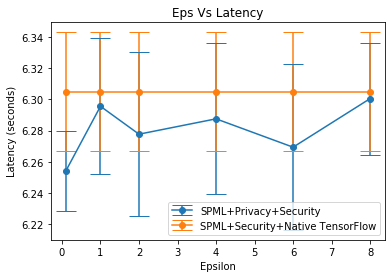
\includegraphics[width=\textwidth]{images/Inference/Cifar10HwLatencyInference.png}
         \caption{Latency}
         \label{fig:hwCifar10LatencyInference}
     \end{subfigure}
        \caption{Cifar10 Dataset - Inference - Hardware mode with Intel SGX and SCONE}
\end{figure}
\newline
\newline
\textbf{\textit{Latency: }}The figures ~\ref{fig:nativeCifar10LatencyInference}, ~\ref{fig:simCifar10LatencyInference}, ~\ref{fig:hwCifar10LatencyInference} shows the inference latency of all the modes. There is not much difference between the latency of the native TensorFlow (SPML) and DP (SPML+privacy) run. However, hardware mode (SPML+security) is almost showing latency of 5.9 seconds which is 7.5$\times$, 19$\times$ as compared to simulation and native mode (SPML without security) respectively. These latency values are much less than the latency of the training phase. Hence, the inference phase can be used in practice because latency is within an acceptable range. 

\section{Randomized response}
To evaluate the randomized response technique for our system SPML, we have used adult dataset \cite{15}. It contains census data with attributes like age, education, relationship, sex, occupation, etc and using these attributes it predicts if the income of an individual can exceed \$50000/year. We choose the sex and relationship column and made them numerical with 0 or 1 responses. Then we added randomization to this dataset by randomizing the sex and relationship numerical column with the coin flip algorithm as explained in the implementation section ~\ref{sec:implementationRR}. We trained the model on 39040 training samples and 9792 inference samples. We followed the same methodology as explained above but the only difference is we used different epoch values for this such as 0.13, 0.53, 1, 2, 3, 4. For each phase, the final accuracy and latency score is an average of 10 iterations with 50 epochs for each epsilon value. In the next sections, we will discuss the results we got from the training and inference phase.

\subsection{Training Phase}
\textbf{\textit{Accuracy: }} As we can see from Figures ~\ref{fig:nativeRRAccuracyTraining}, ~\ref{fig:simRRAccuracyTraining}, ~\ref{fig:hwRRAccuracyTraining} accuracy fluctuates a lot for each epsilon value. It is hard to conclude any trend, like with noise, we can say that accuracy increases with epsilon value. The accuracy with randomized response, remains between 72\% to 75\%. We get definitely almost comparable accuracy as compared to native TensorFlow in all three modes however no trend can be established between accuracy and espilon value.
\begin{figure}
     \begin{subfigure}{0.5\textwidth}
         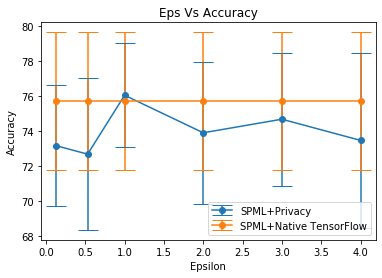
\includegraphics[width=\textwidth]{images/Training/RRAccuracy.png}
         \caption{Accuracy}
         \label{fig:nativeRRAccuracyTraining}
     \end{subfigure}
     \begin{subfigure}{0.5\textwidth}
         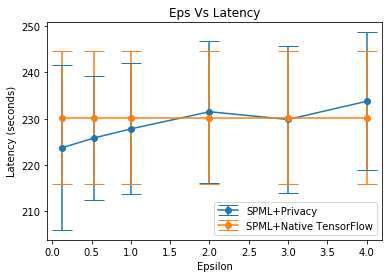
\includegraphics[width=\textwidth]{images/Training/RRLatency.png}
         \caption{Latency}
         \label{fig:nativeRRLatencyTraining}
     \end{subfigure}
        \caption{Randomized response - Training - Native mode without Intel SGX and SCONE}
     \begin{subfigure}{0.5\textwidth}
         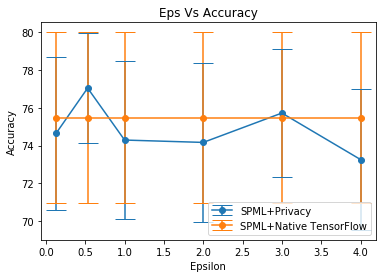
\includegraphics[width=\textwidth]{images/Training/RRSIMAccuracy.png}
         \caption{Accuracy}
         \label{fig:simRRAccuracyTraining}
     \end{subfigure}
     \begin{subfigure}{0.5\textwidth}
         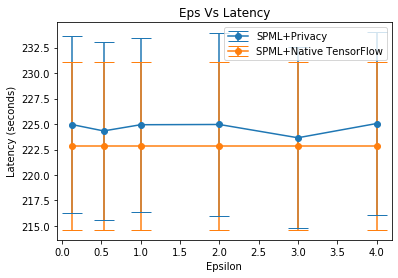
\includegraphics[width=\textwidth]{images/Training/RRSIMLatency.png}
         \caption{Latency}
         \label{fig:simRRLatencyTraining}
     \end{subfigure}
        \caption{Randomized response - Training - Simulation mode without Intel SGX and with SCONE}
        \label{default}
     \begin{subfigure}{0.5\textwidth}
         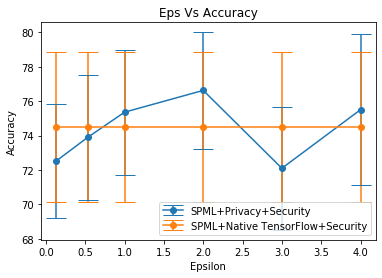
\includegraphics[width=\textwidth]{images/Training/RRHWAccuracy.png}
         \caption{Accuracy}
         \label{fig:hwRRAccuracyTraining}
     \end{subfigure}
     \begin{subfigure}{0.5\textwidth}
         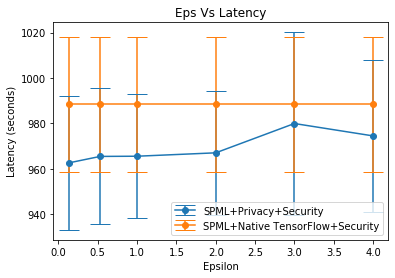
\includegraphics[width=\textwidth]{images/Training/RRHWLatency.png}
         \caption{Latency}
         \label{fig:hwRRLatencyTraining}
     \end{subfigure}
        \caption{Randomized response - Training - Hardware mode with Intel SGX and SCONE}
\end{figure}
\newline
\newline
\textbf{\textit{Latency: }}We can see the Figures in ~\ref{fig:nativeRRLatencyTraining}, ~\ref{fig:simRRLatencyTraining}, ~\ref{fig:hwRRLatencyTraining} for native, simulation, and hardware modes respectively. There is not much difference between native Tensorflow(SPML) and DP(SPML+privacy) run in terms of latency. SPML without privacy and SPML+privacy both have a latency of around 225, 225, 965 seconds for native, simulation, and hardware mode respectively. SPML has a latency of around 225 seconds for native and simulation mode while SPML + security is touching latency of around 965 seconds. After enabling security property in SPML latency is almost 4.2$\times$ as compared to SPML without security.
\subsection{Inference Phase}
\textbf{\textit{Accuracy: }} We can see that accuracy fluctuates a lot for each epsilon value in our system SPML for inference also as can be seen in Figures ~\ref{fig:nativeRRAccuracyInference}, ~\ref{fig:simRRAccuracyInference}, ~\ref{fig:hwRRAccuracyInference} . As discussed in the training phase, it is hard to conclude any trend here. The accuracy values are between 80\% and 82\%. We get definitely almost comparable accuracy as compared to native TensorFlow in all three modes however no trend can be established between accuracy and epsilon value.
\begin{figure}
     \begin{subfigure}{0.5\textwidth}
         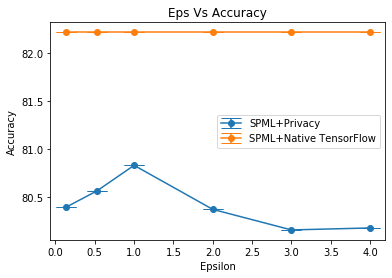
\includegraphics[width=\textwidth]{images/Inference/RRAccuracy.png}
         \caption{Accuracy}
         \label{fig:nativeRRAccuracyInference}
     \end{subfigure}
     \begin{subfigure}{0.5\textwidth}
         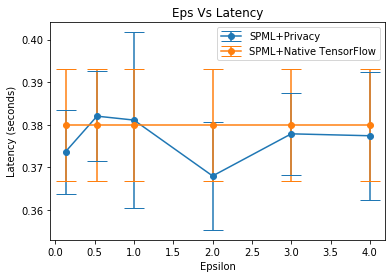
\includegraphics[width=\textwidth]{images/Inference/RRLatency.png}
         \caption{Latency}
         \label{fig:nativeRRLatencyInference}
     \end{subfigure}
        \caption{Randomized response - Inference - Native mode without Intel SGX and SCONE}
     \begin{subfigure}{0.5\textwidth}
         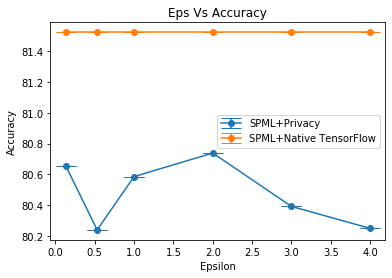
\includegraphics[width=\textwidth]{images/Inference/RRSIMAccuracy.png}
         \caption{Accuracy}
         \label{fig:simRRAccuracyInference}
     \end{subfigure}
     \begin{subfigure}{0.5\textwidth}
         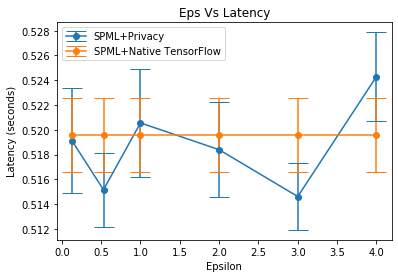
\includegraphics[width=\textwidth]{images/Inference/RRSIMLatency.png}
         \caption{Latency}
         \label{fig:simRRLatencyInference}
     \end{subfigure}
        \caption{Randomized response - Inference - Simulation mode without Intel SGX and with SCONE}
     \begin{subfigure}{0.5\textwidth}
         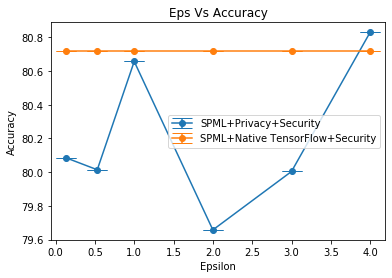
\includegraphics[width=\textwidth]{images/Inference/RRHWAccuracy.png}
         \caption{Accuracy}
         \label{fig:hwRRAccuracyInference}
     \end{subfigure}
     \begin{subfigure}{0.5\textwidth}
         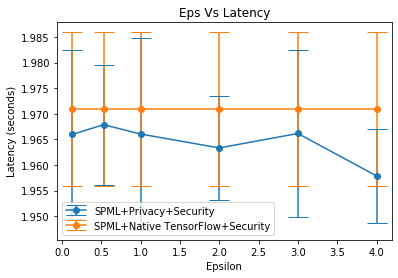
\includegraphics[width=\textwidth]{images/Inference/RRHWLatency.png}
         \caption{Latency}
         \label{fig:hwRRLatencyInference}
     \end{subfigure}
        \caption{Randomized response - Inference - Hardware mode with Intel SGX and SCONE}
\end{figure}
\newline
\newline
\textbf{\textit{Latency: }}We can see the latency values in Figure ~\ref{fig:nativeRRLatencyInference}, ~\ref{fig:simRRLatencyInference}, ~\ref{fig:hwRRLatencyInference} . SPML without privacy and SPML+privacy has the same latency of around 0.32 seconds for native mode. SPML has a latency of around 0.52 seconds for simulation mode while SPML + security is touching latency of around 1.95 seconds. After enabling security property in SPML latency is almost 6$\times$ as compared to SPML without security. Hence, the inference phase is much faster for our system SPML as compare to the training phase for randomized response also.

We have already seen MNIST and CIFAR10 dataset results already as well as randomized responses, in the discussion section ~\ref{sec:evalDiscussion}, we will summarize what we have learned from the measurements and what can be concluded about these runs and different modes. Before discussing the results, in the next section we have evaluated our system SPML against one of the machine learning attack to see visually the application of SPML.

\section{Machine learning attack}
\label{sec:evalMLAttack}
We also evaluated our system SPML against model inversion attack \cite{17} to proof our work. The model inversion attack as defined in \cite{17} states, if an adversary has access to a trained model and some auxiliary information about an individual, then it can make predictions about an individual’s genetic markers. This particular attack is discussed via an example from the pharmacogenetics field in the paper, but it can be generalized in any scenario like we have used this type of attack on the classification of hand-written digits from MNIST \cite{12} dataset.
\begin{figure}
     \begin{subfigure}{.325\textwidth}
         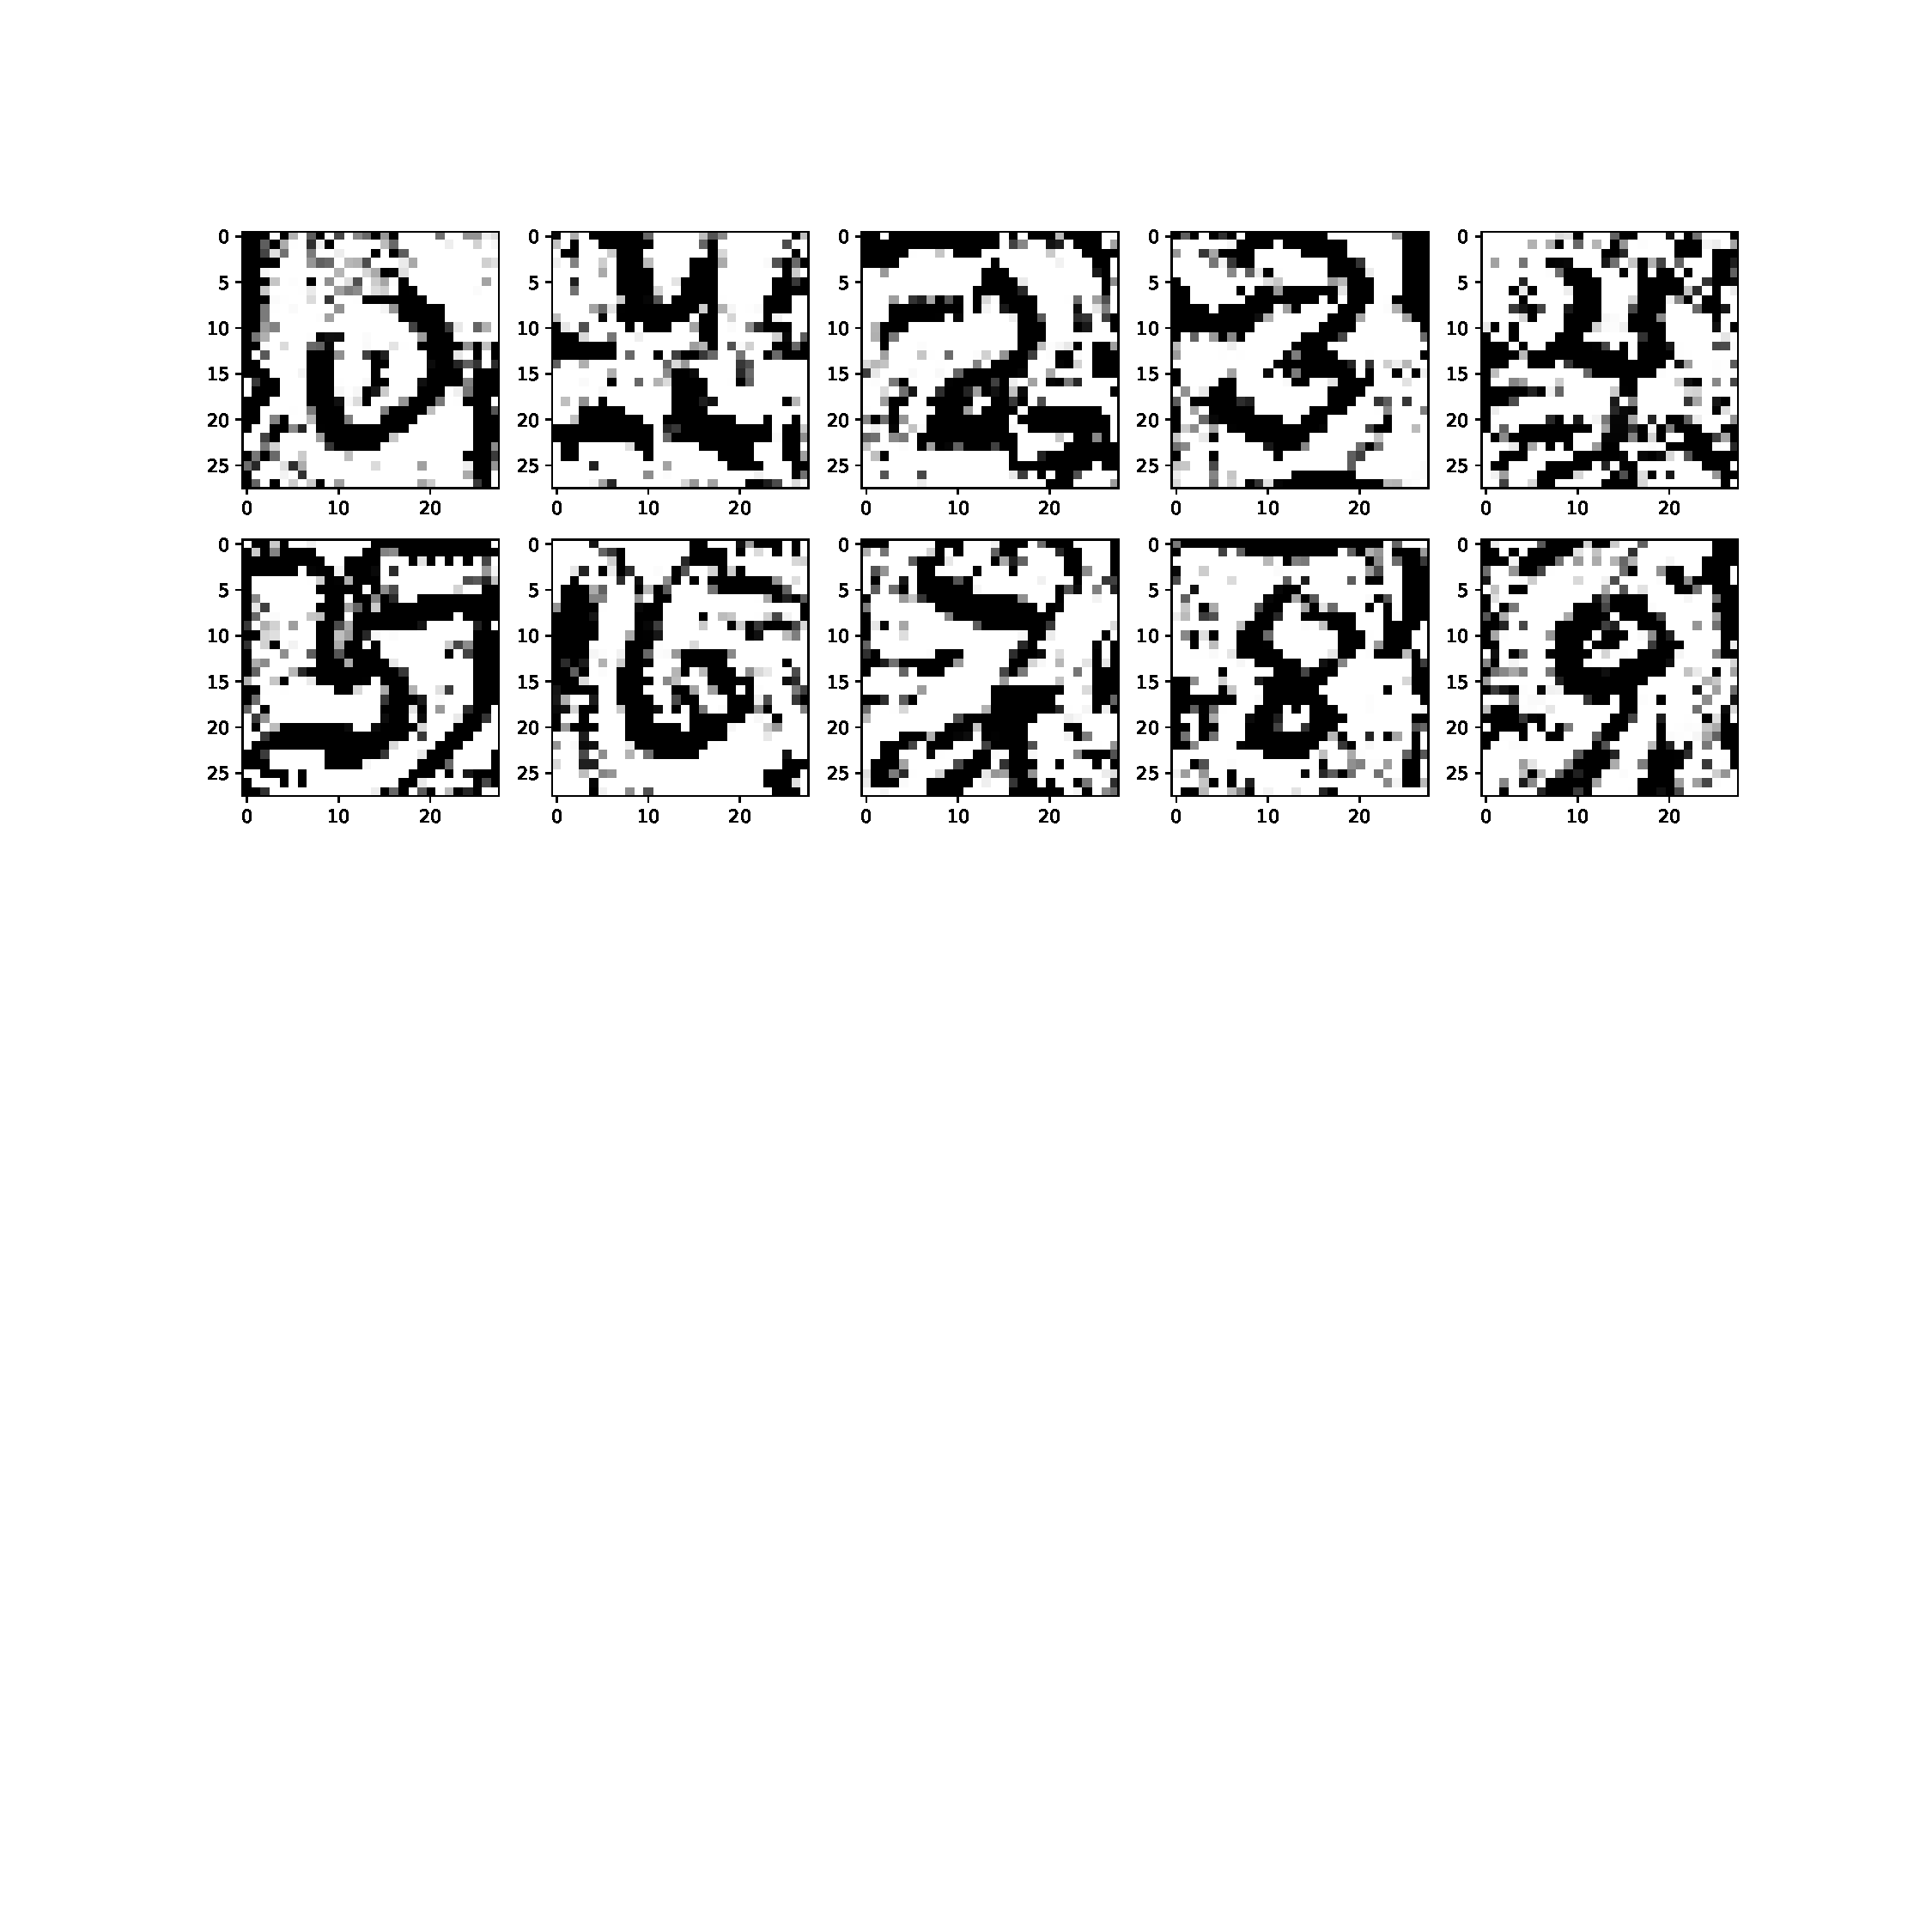
\includegraphics[width=\textwidth]{images/Native_attack/Mnistattack_native.pdf}
         \vspace{-8em}
         \caption{SPML+Native TensorFlow; and, Accuracy=99.55\%}
         \label{fig:nativeEps0}
     \end{subfigure}
     \begin{subfigure}{.325\textwidth}
         \includegraphics[width=\textwidth]{images/Native_attack/Mnistattack.2.pdf}
         \vspace{-8em}
         \caption{SPML+Privacy; $\epsilon$=0.2; and, Accuracy=10.12\%;}
         \label{fig:nativeEps.2}
     \end{subfigure}
     \begin{subfigure}{.325\textwidth}
         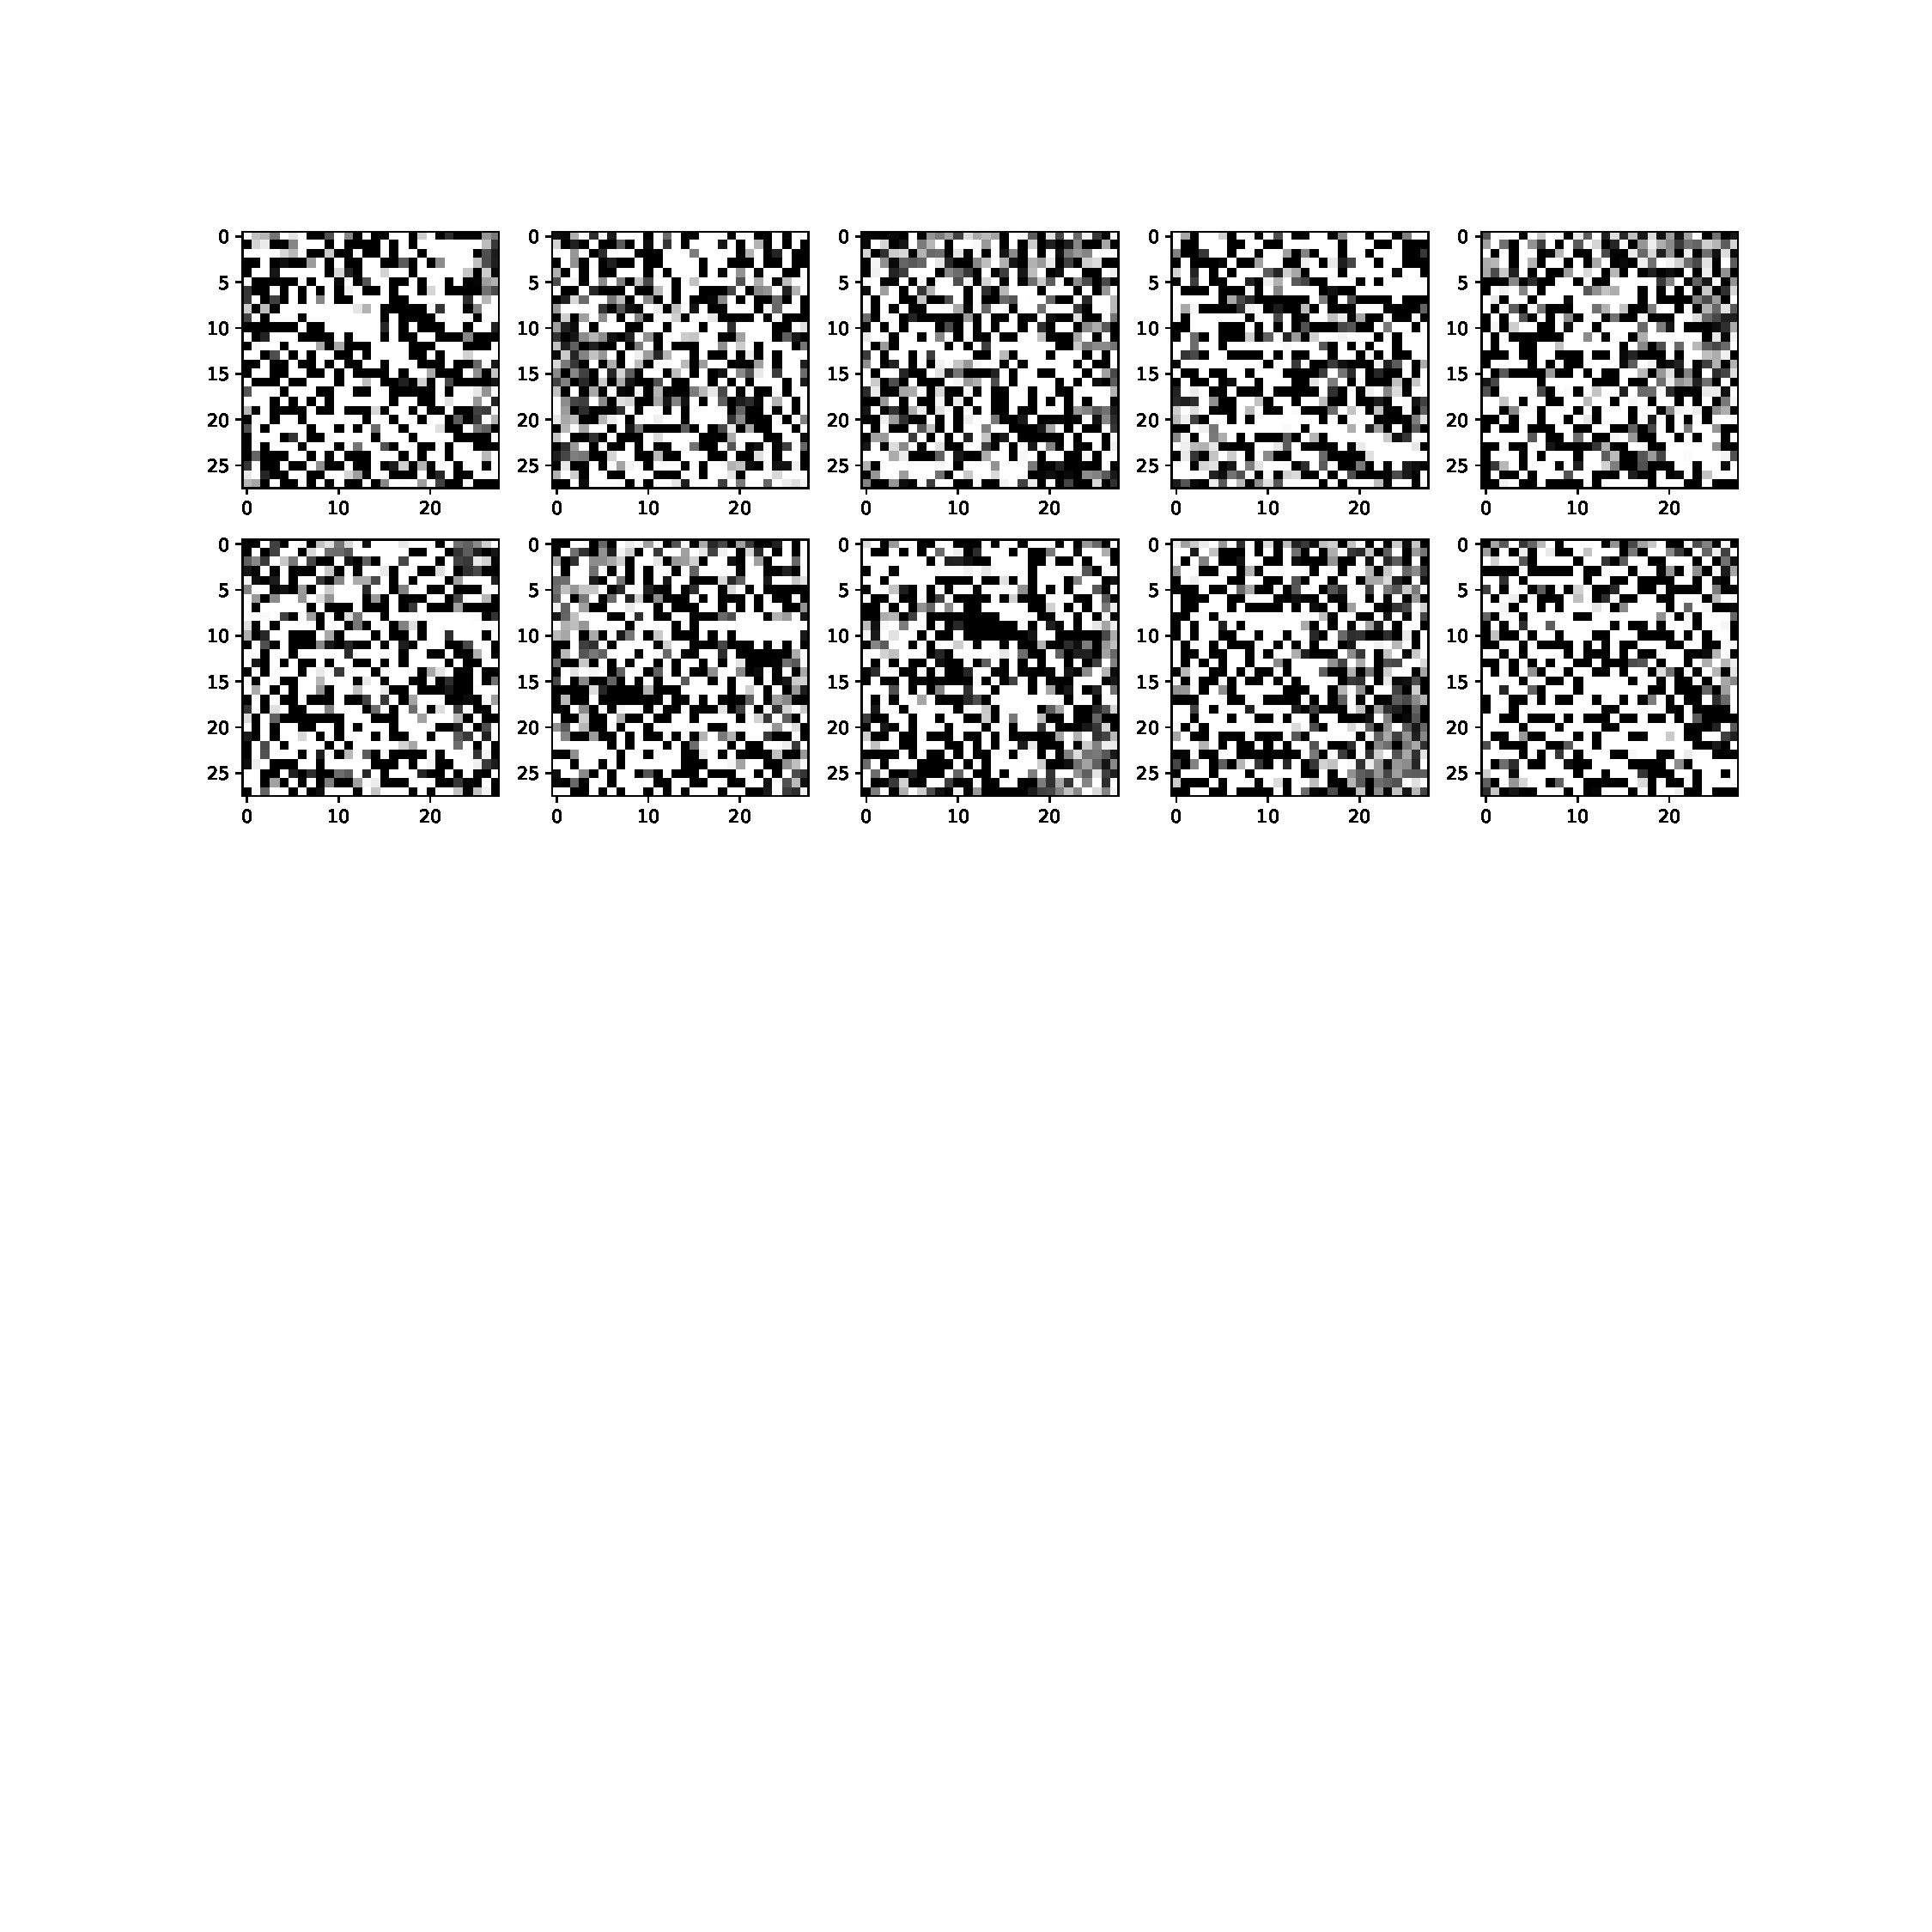
\includegraphics[width=\textwidth]{images/Native_attack/Mnistattack8.pdf}
         \vspace{-8em}
         \caption{SPML+Privacy; $\epsilon$=8; and, Accuracy=85.36\%;}
         \label{fig:nativeEps8}
     \end{subfigure}
        \caption{Model inversion attack images - Native mode without Intel SGX and SCONE}
%\end{figure}
%\begin{figure}
     \begin{subfigure}{.325\textwidth}
         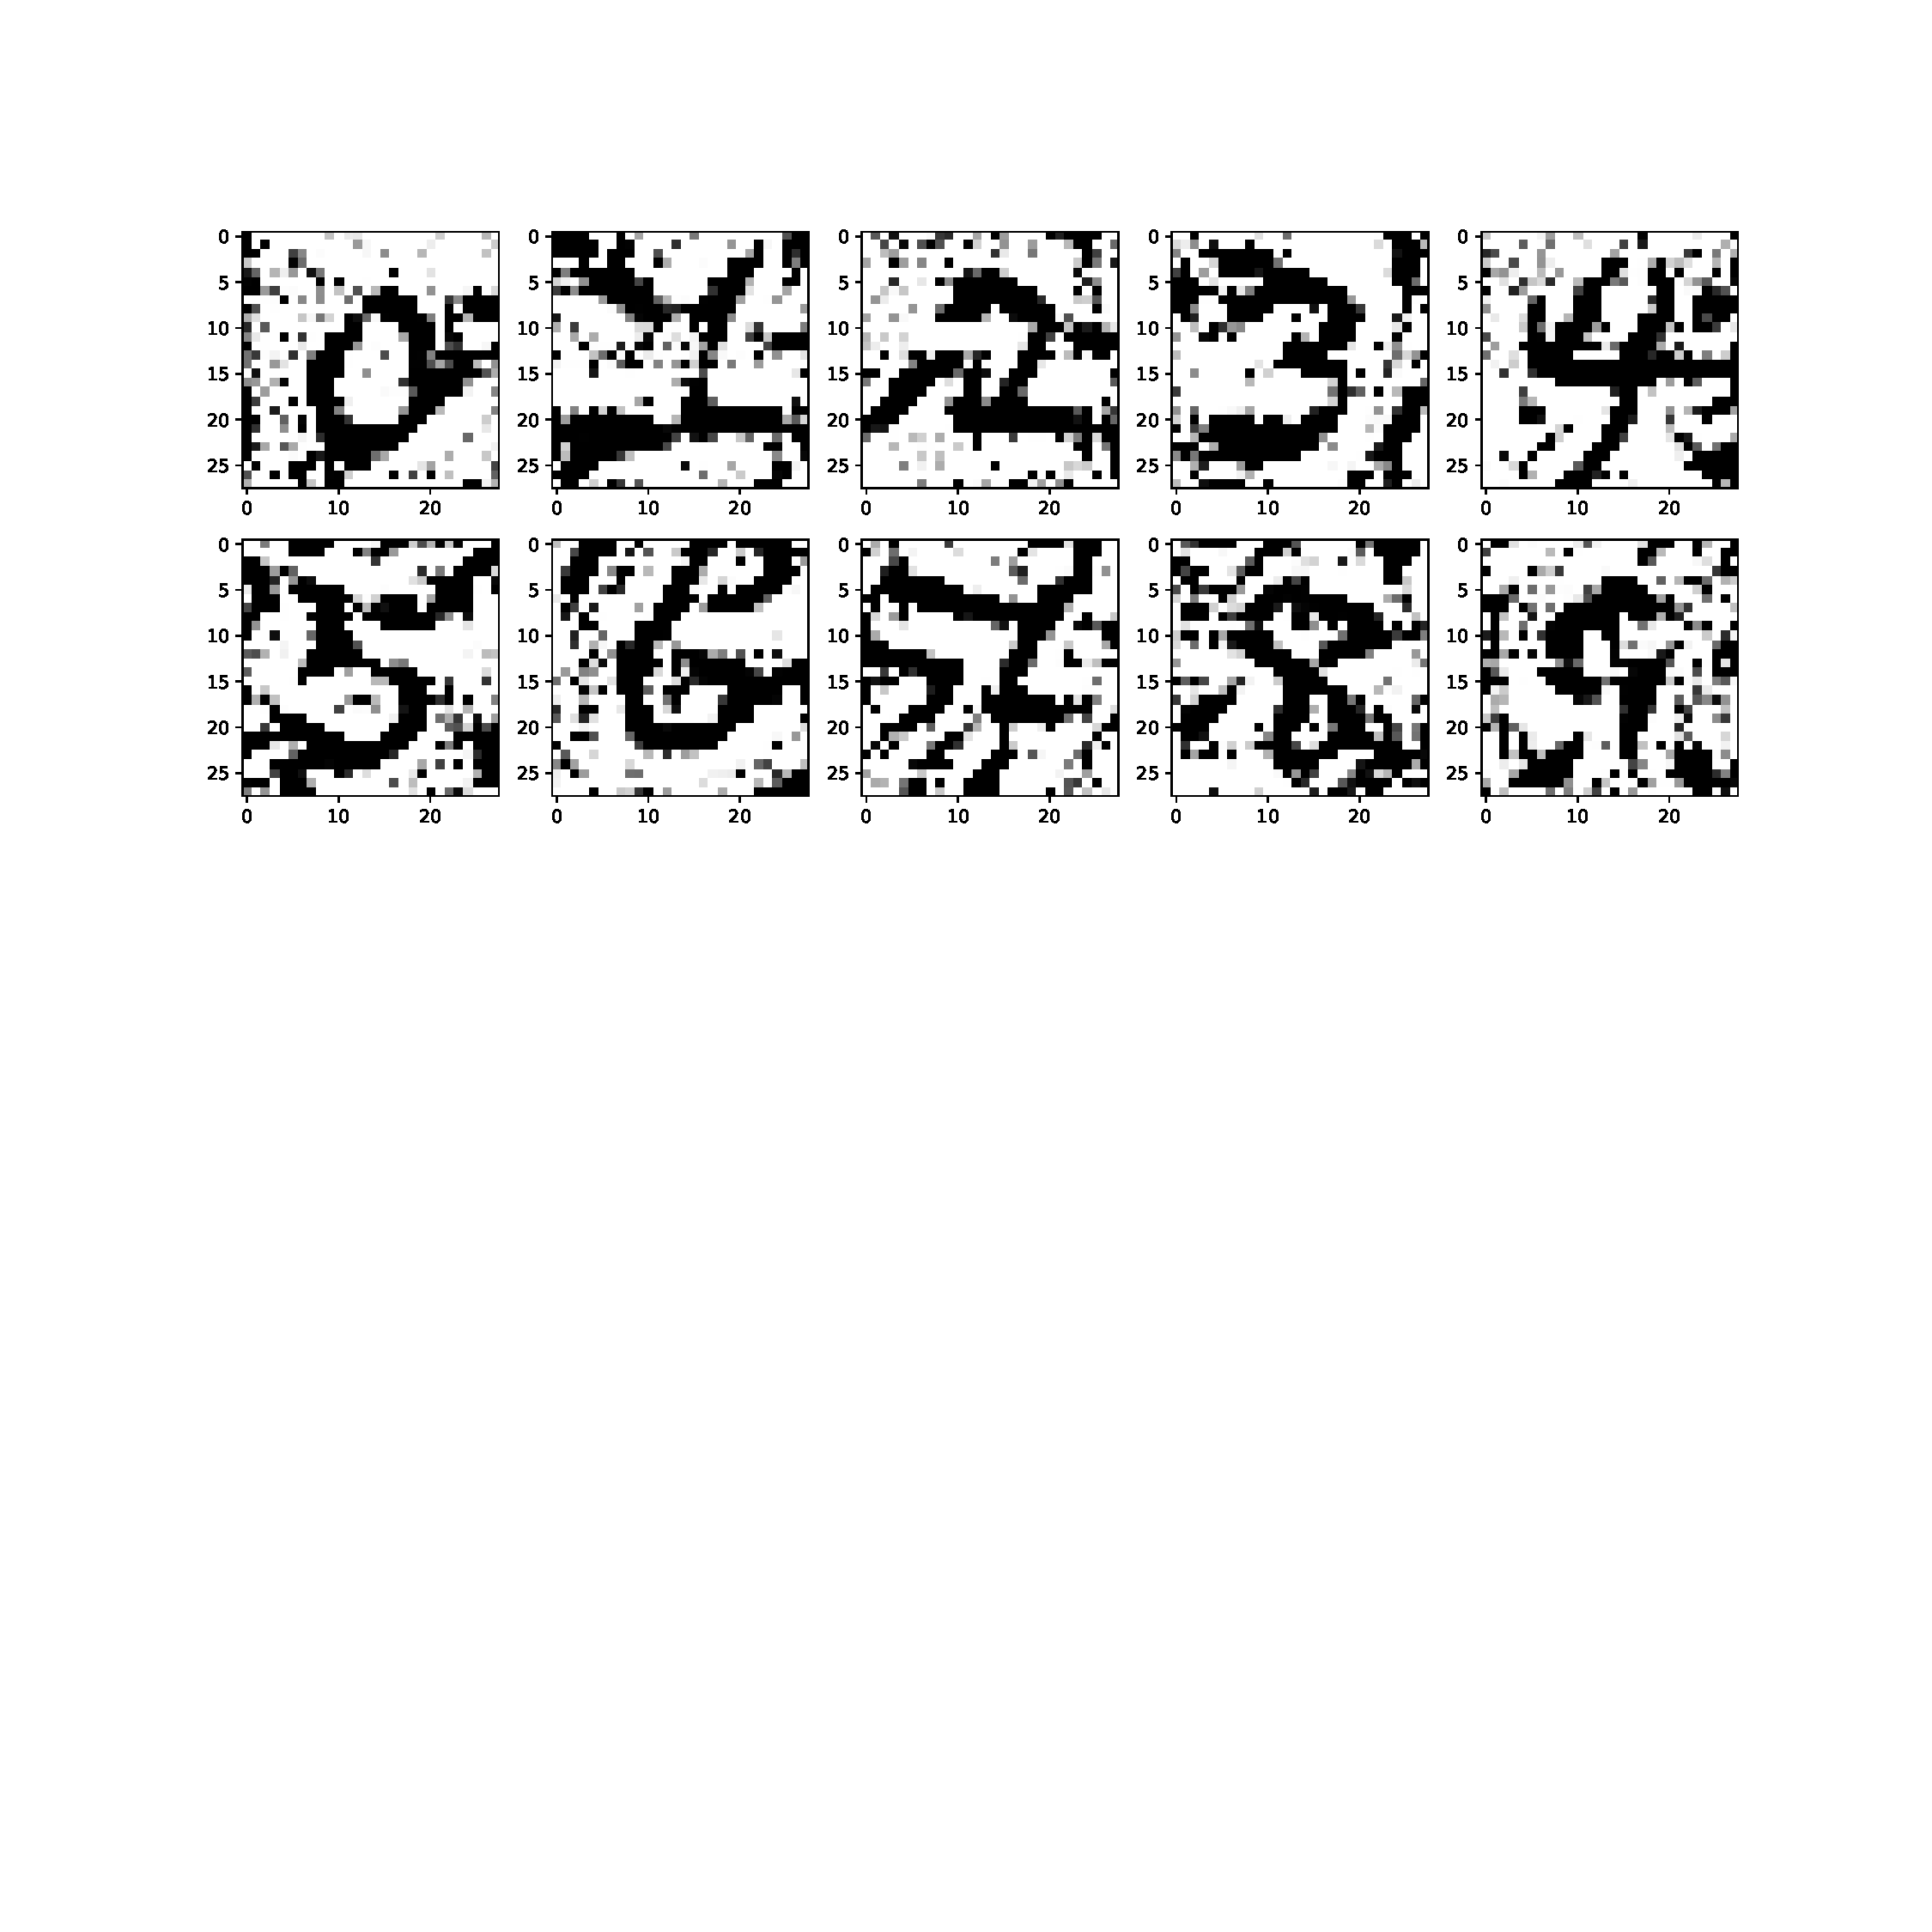
\includegraphics[width=\textwidth]{images/Sim_attack/Mnistattack_native.pdf}
         \vspace{-8em}
         \caption{SPML+Native TensorFlow; and, Accuracy=99.72\%}
         \label{fig:simEps0}
     \end{subfigure}
     \begin{subfigure}{.325\textwidth}
         \includegraphics[width=\textwidth]{images/Sim_attack/Mnistattack.2.pdf}
         \vspace{-8em}
         \caption{SPML+Privacy; $\epsilon$=0.2; and, Accuracy=11.66\%;}
         \label{fig:simEps.2}
     \end{subfigure}
     \begin{subfigure}{.325\textwidth}
         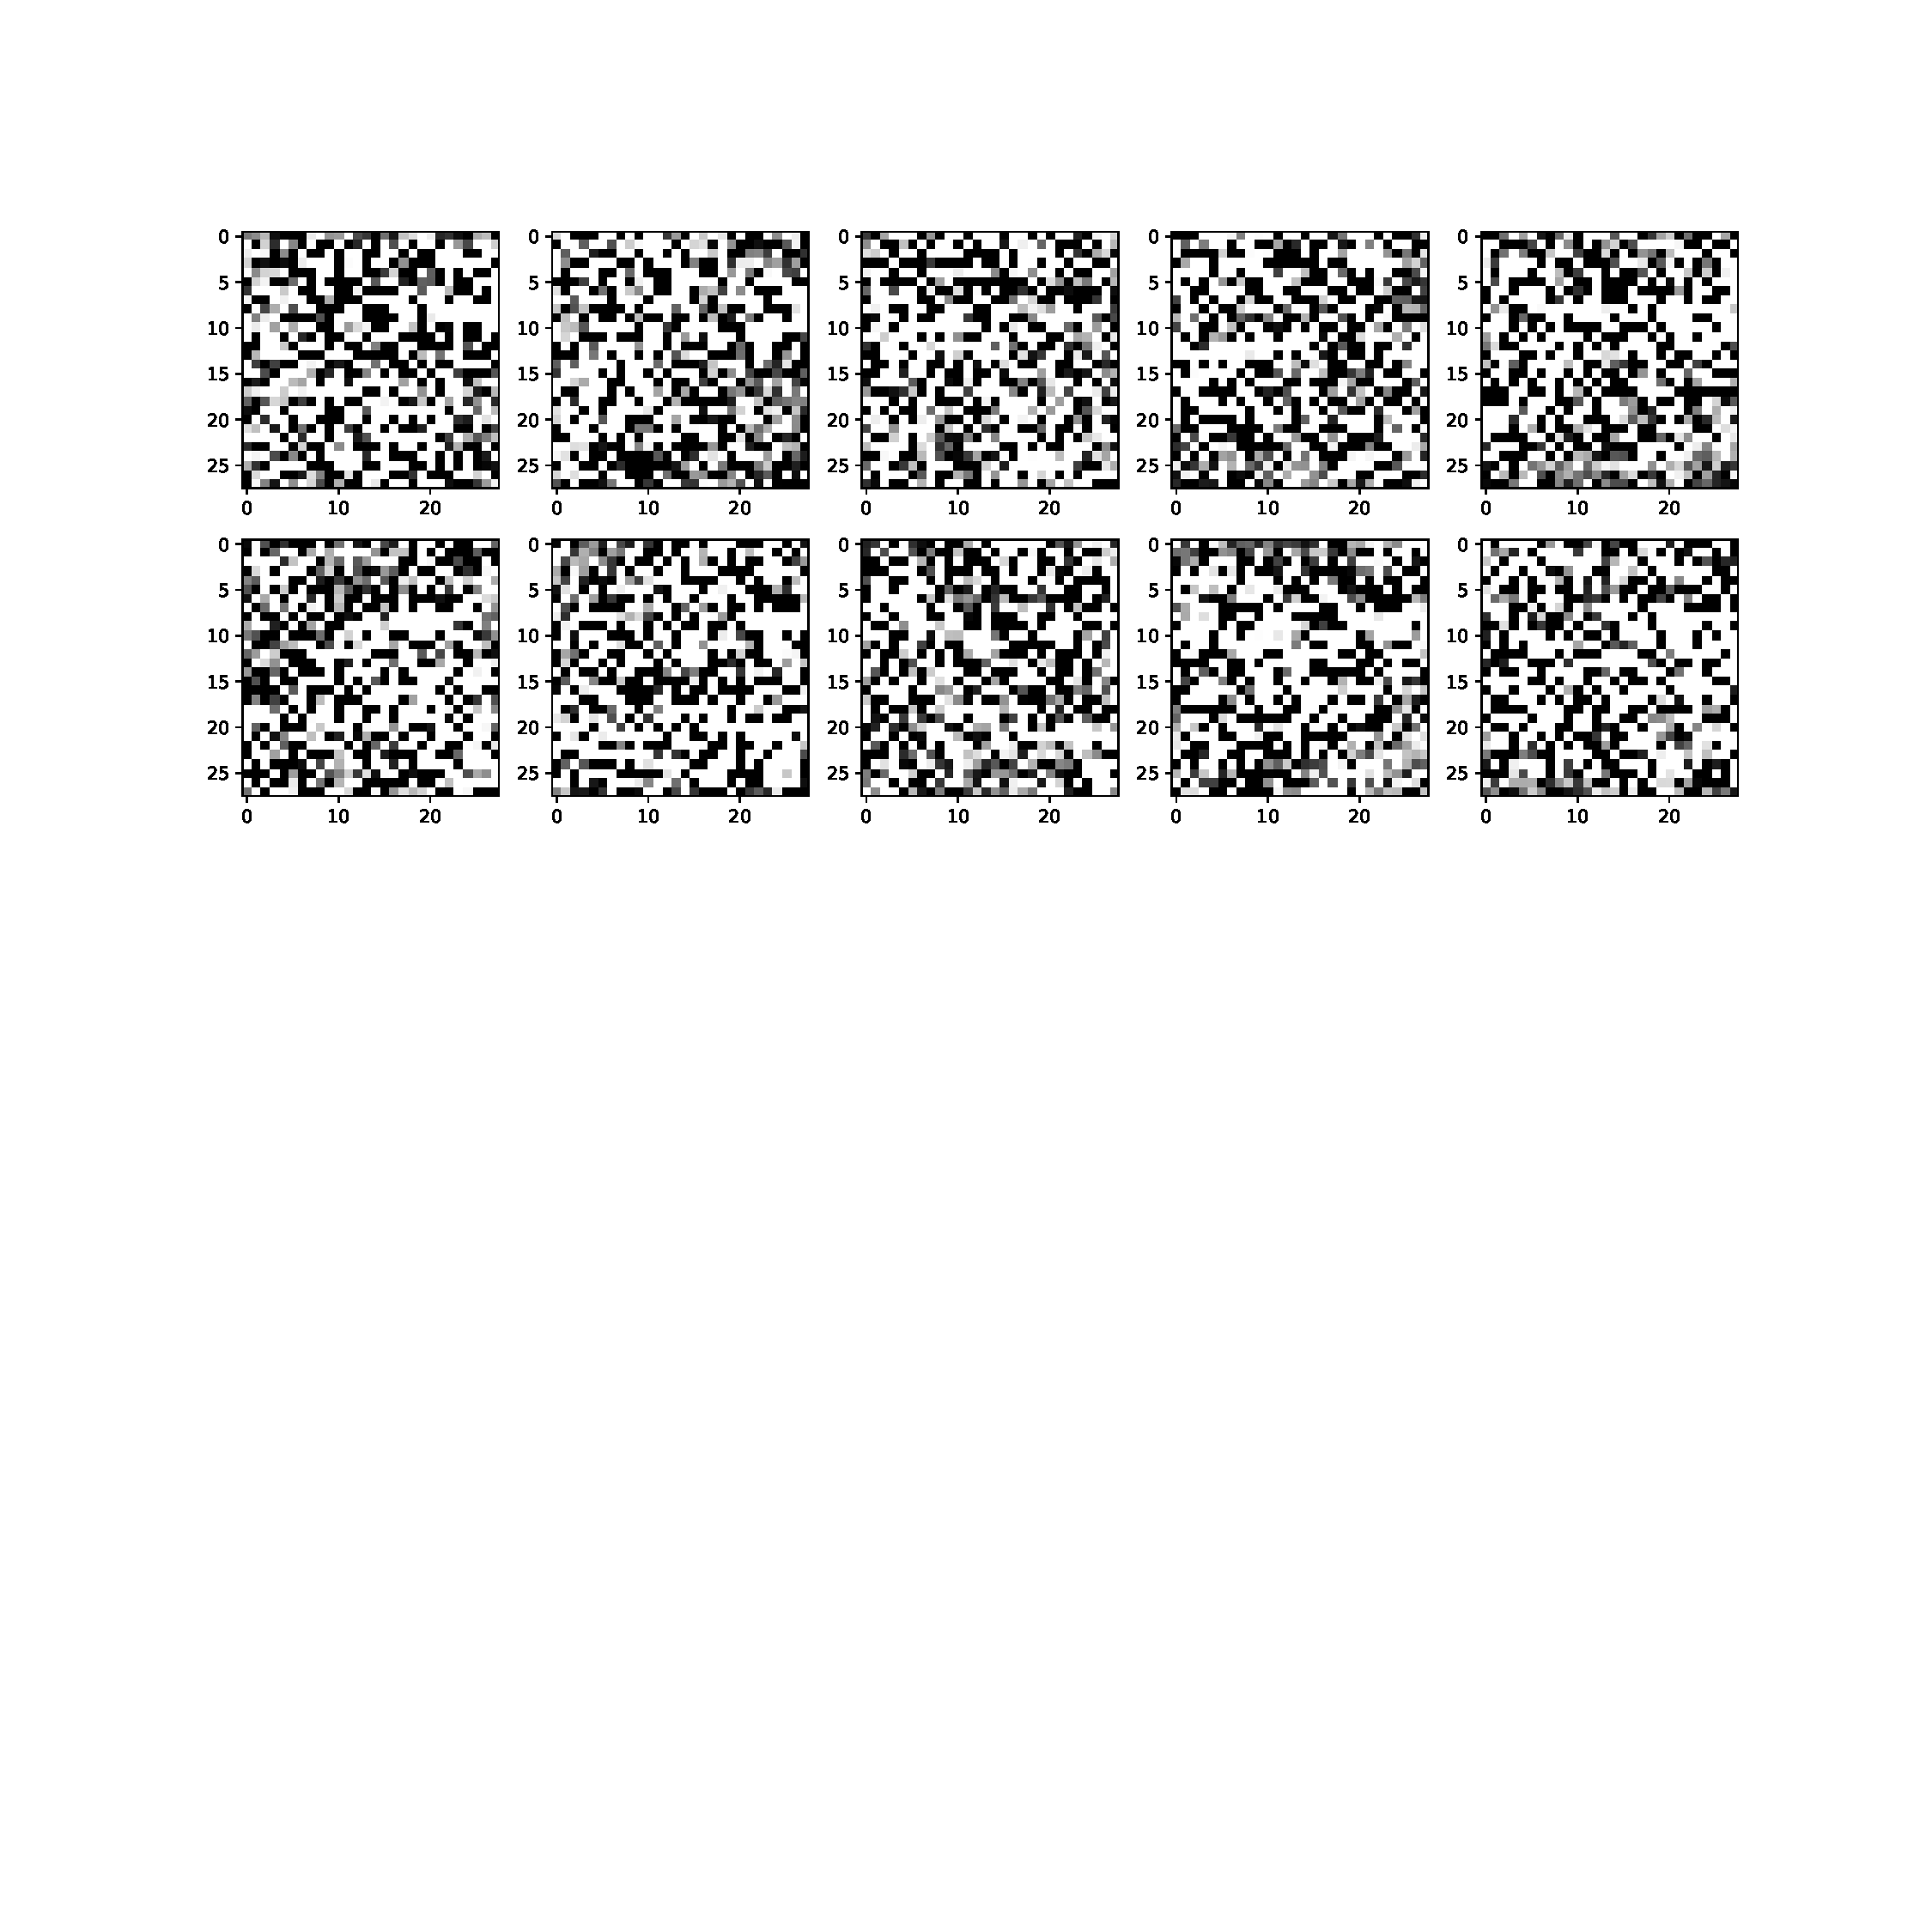
\includegraphics[width=\textwidth]{images/Sim_attack/Mnistattack8.pdf}
         \vspace{-8em}
         \caption{SPML+Privacy; $\epsilon$=8; and, Accuracy=84.37\%;}
         \label{fig:simEps8}
     \end{subfigure}
        \caption{Model inversion attack images - Simulation mode without Intel SGX and with SCONE}
%\end{figure}
%\begin{figure}
     \begin{subfigure}{.325\textwidth}
         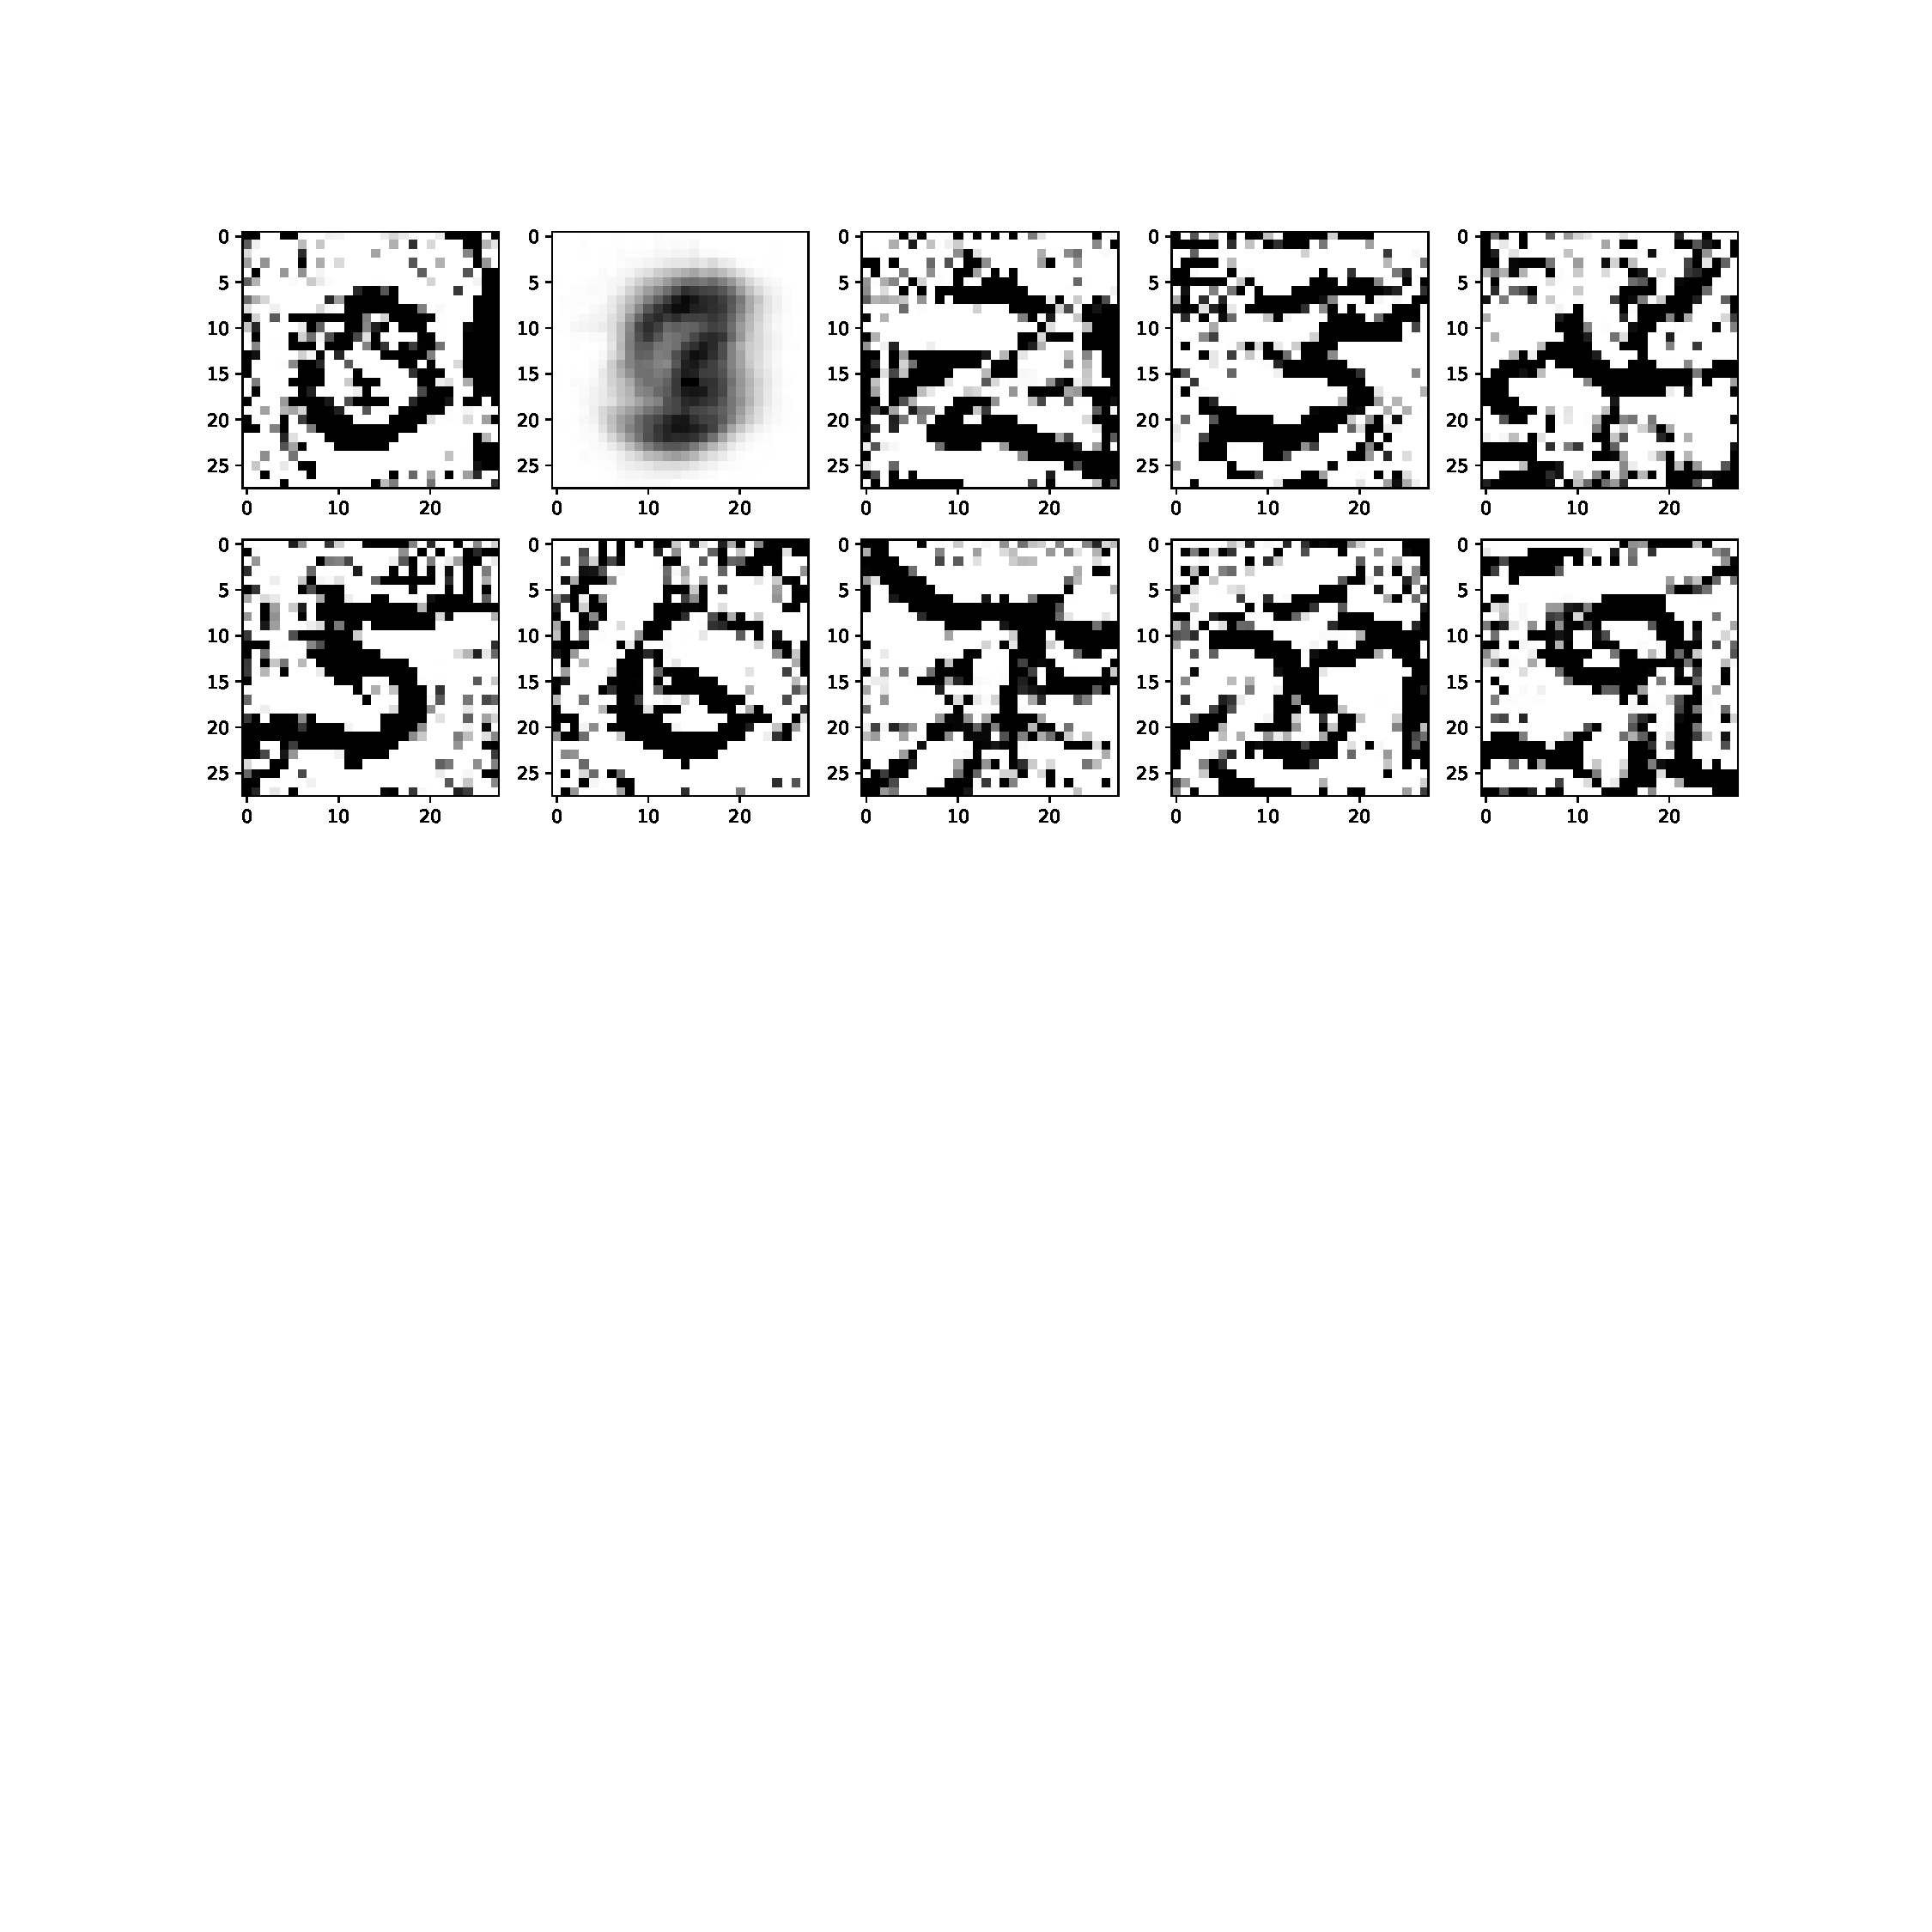
\includegraphics[width=\textwidth]{images/Hw_attack/Mnistattack_native.pdf}
         \vspace{-8em}
         \caption{SPML+Native TensorFlow; and, Accuracy=99.65\%}
         \label{fig:hwEps0}
     \end{subfigure}
     \begin{subfigure}{.325\textwidth}
         \includegraphics[width=\textwidth]{images/Hw_attack/Mnistattack.2.pdf}
         \vspace{-8em}
         \caption{SPML+Privacy; $\epsilon$=0.2; and, Accuracy=10.19\%;}
         \label{fig:hwEps.2}
     \end{subfigure}
     \begin{subfigure}{.325\textwidth}
         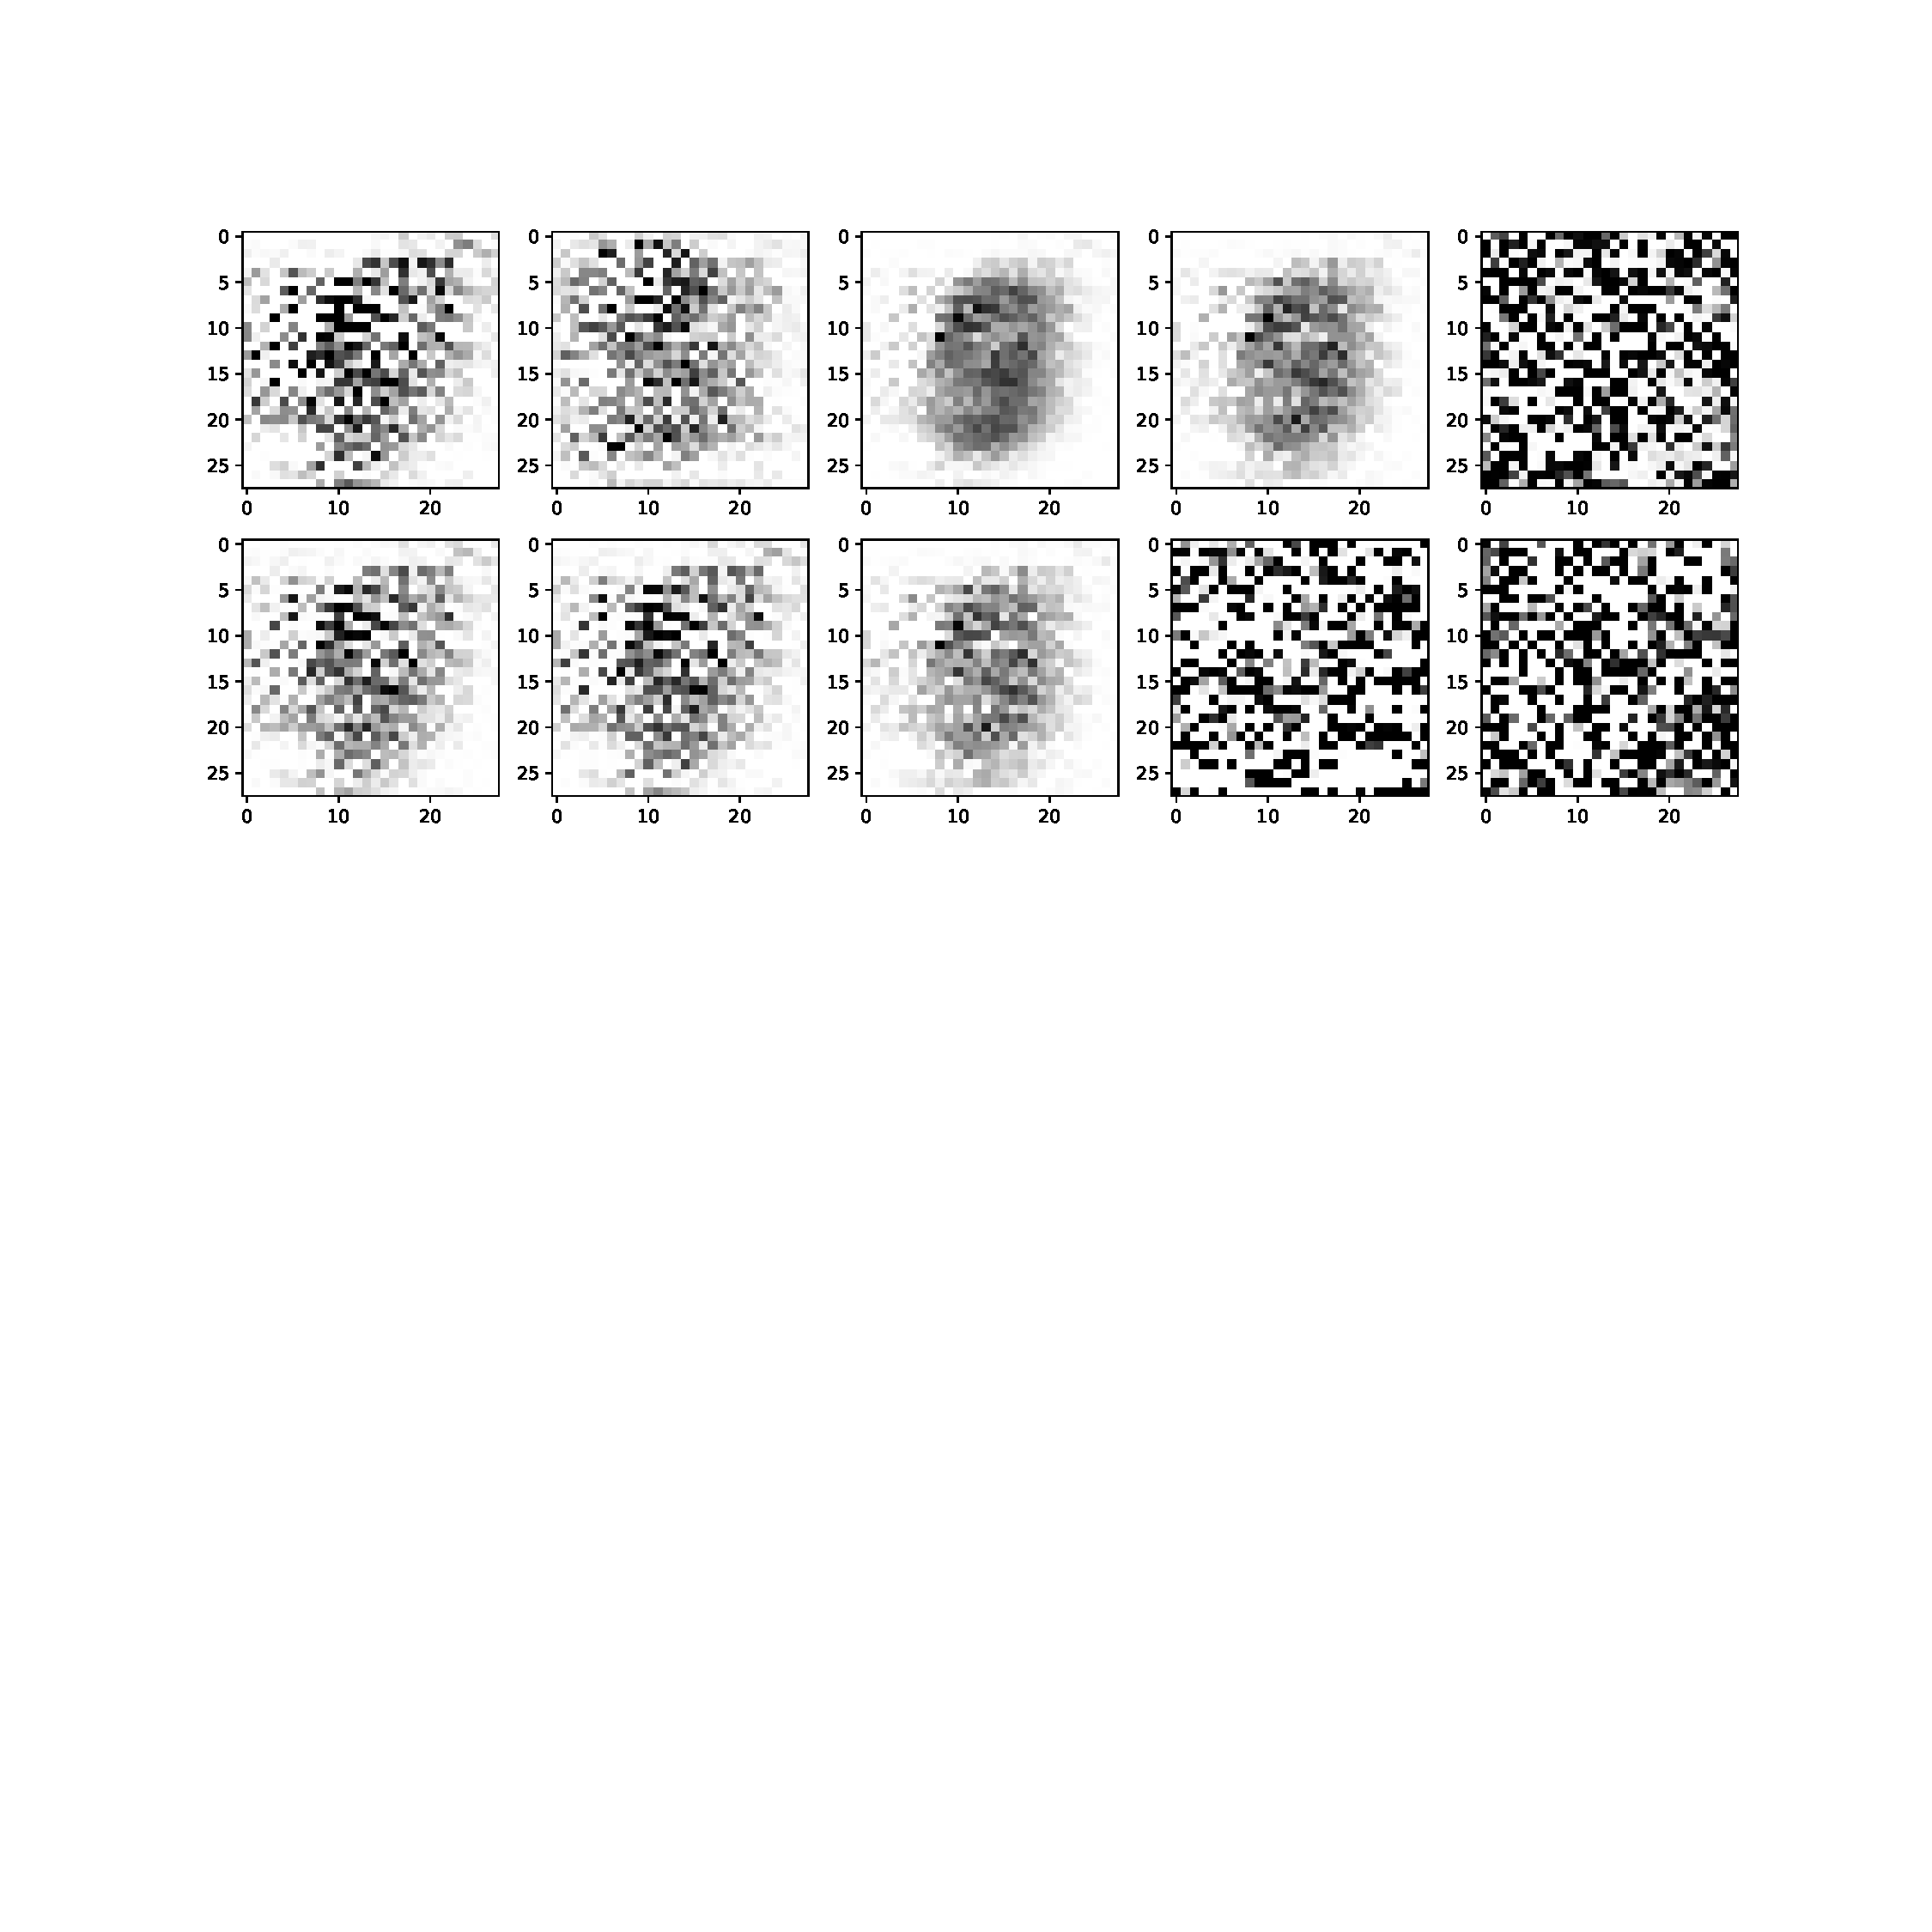
\includegraphics[width=\textwidth]{images/Hw_attack/Mnistattack8.pdf}
         \vspace{-8em}
         \caption{SPML+Privacy; $\epsilon$=8; and, Accuracy=85.93\%;}
         \label{fig:hwEps8}
     \end{subfigure}
        \caption{Model inversion attack images - Hardware mode with Intel SGX and SCONE}
\end{figure}
To implement this attack \footnote{https://github.com/prbh695a/SPML/tree/master/Model\%20Inversion\%20attack}, we have used IBM's open-source Adversarial Robustness Toolbox (ART) \cite{76} library. The model is trained with the MNIST dataset with 60,000 training samples. We have used 10,000 test samples as explained in the library for better visualization. We have assumed the mean values of test data for each digit as the auxiliary information for our evaluation. We used epsilon values as 0.2, 1, 2, 4, 6, 8 in all three modes which are native mode (i.e without Intel SGX and SCONE), SCONE simulation mode, and SCONE hardware mode.

In all the modes (i.e native, SCONE simulation, and SCONE hardware), the attack is executed on SPML+Native TensorFlow and SPML+Privacy. We enable privacy property in all three modes, and security property is enabled in SCONE hardware mode only. When the attack was done on the SPML+Native TensorFlow trained model, we can see that in Figure ~\ref{fig:nativeEps0}, ~\ref{fig:simEps0}, ~\ref{fig:hwEps0}, that many of the digits are revealed and we can take hints what kind of training data was used. Hence, our attack is successful. Therefore, without enabling privacy property individual training data is leaked. SPML aims to protect individual's information by enabling privacy property to prevent such types of attacks.

The privacy property is enabled for different epsilon values as 0.2, 1, 2, 4, 6, 8. For the discussion purpose, we will be discussing epsilon values 0.2 and 8 only, as the rest of the epsilon values showed almost the same results. However, for completeness, the detailed images for all the trained models with different epsilon values are shown in ~\ref{sec:MIA}. When the attack was executed on the model trained with epsilon value 8 with our system SPML, as shown in Figure ~\ref{fig:nativeEps8}, ~\ref{fig:simEps8}, ~\ref{fig:hwEps8} then we are not able to make out any of the images used in the training set.  The trained model with epsilon value 8 has an accuracy of almost 85 percent but still, we cannot visualize the images clearly because we have enabled privacy property in our system SPML.

The model trained with epsilon value from 0.2 to 4 achieved an accuracy of around 10-11\% hence these models cannot be used for classification in practice. Visually also, the images are not usable as shown in Figure ~\ref{fig:nativeEps.2}, ~\ref{fig:simEps.2}, ~\ref{fig:hwEps.2}. Hence, the privacy property and accuracy have a trade-off which we should make. The trade-off can be seen graphically and mathematically in sections ~\ref{sec:evalMnist} and ~\ref{sec:evalCifar10} and this section proves this trade-off visually. 

We can conclude that our system SPML not only protects the confidentiality and integrity of the system but it also avoids leakage of private and sensitive information of the individuals participating in the training dataset. 

\section{Discussion}
\label{sec:evalDiscussion}
In this section, we will discuss how our system SPML system performed in terms of accuracy and latency. We will be using the measurement from the MNIST, CIFAR10 dataset as seen above. This section is divided into two parts to study the effect of (1) Privacy (2) Confidentiality and integrity property. Privacy is achieved using differential privacy which is implemented using TensorFlow privacy library \cite{11} or randomized response. Confidentiality and integrity are achieved using Intel SGX and integration is done using SCONE runtime environment. We will first discuss the effect of enabling only privacy and then the effect of enabling both privacy and security in our system SPML with noise and in the next subsection we will discuss randomized response separately.

\subsection{Privacy:} 
When privacy is added to the data, we aim to protect the individual's information from any kind of leakage that could happen via attacks as discussed in the background chapter ~\ref{sec:attackOnML}. To implement privacy, we are using the TensorFlow privacy library which uses differential privacy techniques to add privacy. In this library, random Gaussian noise is added during the training of the model.
\newline
\newline
\textbf{\textit{Training phase: }}For the training phase, when we add only privacy to the system the accuracy increases with epsilon value as seen in Figure ~\ref{fig:nativeMnistAccuracyTraining}. However, latency for DP(SPML+privacy) run is almost 10$\times$ higher than the native TensorFlow(SPML) run for MNIST as shown in ~\ref{fig:nativeMnistLatencyTraining}. This is the cost of adding privacy in our system SPML. One has to bear this cost if the privacy-preserving system is needed using the TensorFlow privacy library.
\newline
\newline
\textbf{\textit{Inference phase: }}On the other hand if we look at the results of the inference phase, then accuracy holds the same notion as discussed above, which is accuracy increases with epsilon value as seen in Figure ~\ref{fig:nativeMnistAccuracyInference}. The latency of the inference phase is almost the same for both runs i.e with and without privacy. This is one of the advantages of our system, that inference latency is not affected by the addition of privacy. In terms of productivity, we can say that once the model is trained, an inference can be done in normal working hours with no or very less wait times, however training should be planned in advance due to high training time. After discussing privacy property, we want to discuss security property affect on SPML.

\subsection{Confidentiality and Integrity}
When we add confidentiality and integrity to an application/system we have to use encryption and decryption. This means data, code, and model will be in encrypted form and before executing in an enclave this will be decrypted. The same thing is applicable for the output, it will be decrypted inside an enclave and will be encrypted when it will be saved on the disk (outside an enclave). This encryption/decryption will be adding additional overhead for any system/application where confidentiality and integrity have to be added. We have used the SCONE runtime environment which enables us to use TEEs easily and transparently. For TEEs, we have used Intel SGX for our system SPML. We will first discuss the training phase and then the inference phase for accuracy and latency for SPML.
\newline
\newline
\textbf{\textit{Training phase: }}For the training phase, accuracy is not affected a lot when we add confidentiality and integrity to the data, code, and model as seen in Figure ~\ref{fig:hwMnistAccuracyTraining}. The accuracy is affected only by enabling privacy property as discussed above, enabling security property is not affecting accuracy. It remains almost comparable to native and simulation mode for both the native TensorFlow (SPML+native TensorFlow) and DP runs (SPML+privacy). However, latency, as expected, degraded a lot after enabling security property. In the hardware mode, the native TensorFlow (SPML+security) run has a latency of almost 10$\times$ as compared to native mode (SPML). On the other hand, DP (SPML+security+privacy) runs have a latency of almost 25$\times$ as compared to native (SPML+privacy) mode. Hence, it's not possible to train models in working hours, we have to plan nightly or weekend runs for training the models after enabling security and privacy property.
\newline
\newline
\textbf{\textit{Inference phase: }}For the inference phase, the accuracy trend remains same as discussed above in the training phase. The security property is not affecting accuracy. The latency remains the same for native TensorFlow(SPML+security) and DP(SPML+privacy+security) run in hardware mode. For hardware mode (SPML+security+privacy) latency is 6$\times$ times  than the native mode (SPML+privacy). Inference latency is within the acceptable limit and hence can be used in practice. 

We can conclude that privacy property is affecting both the evaluation parameters which is accuracy and latency for SPML. At the strong privacy bounds which is at low epsilon values, the accuracy is very low and at weaker privacy bounds which is at higher epsilon values accuracy is acceptable. As seen, from the figures of the attack ~\ref{fig:nativeEps0}, ~\ref{fig:nativeEps.2} and ~\ref{fig:nativeEps8}, models trained with high epsilon values can be used in practice and they provide privacy also. The is the trade off we have discussed between the privacy and accuracy level. It is left to the individual how they want to apply this trade off in their respective applications or systems. On the other hand, security property only affects latency parameter. Accuracy is independent of security property. Hence we can control the accuracy level in SPML according to our requirement. Therefore, if we enable both the properties in SPML, then we have to pay the cost of enabling these properties in terms of only latency and to an extent accuracy and we get important properties like privacy, confidentiality and integrity.

\subsection{Randomized response}
The advantage of using randomized noise is that each user can make their data differentially private while filling up the responses for the survey or during data collection. It enables the user to have plausible deniability. However, when it is used on the training dataset, though it makes models differentially private, another parameter such as accuracy is hard to depict. Sometime it may result in better accuracy than a native algorithm or sometimes worse as seen in the above Figures ~\ref{fig:nativeRRAccuracyTraining}, ~\ref{fig:simRRAccuracyTraining} and ~\ref{fig:hwRRAccuracyTraining}. This is because the datapoint in data can be changed as a whole which makes the dataset entirely different. After looking above measurement we can conclude that no trend can be exactly said for accuracy and epsilon values, however, latency is not affected much by enabling privacy property it remains the same. Latency is deteriorated 4.2$\times$, 5.2$\times$ for training and inference phase respectively for enabling security property as compare to without security property. Hence, in practice, we can use inference as well as training for this type of technique. However, we need a way to make it more generalize as it can be only applied to statistical survey techniques for making predictions. For classification problems (image or object), it may need more work. 

Hence, it is better to use SPML and achieve differential privacy with noise as it can be used to predict as well as classify and very few changes are required in the existing system. There is a clear trend for accuracy and we have more control over how much noise should be added as opposed to a randomized response where it is hard to establish a clear trend between accuracy and epsilon value. SPML system takes more time for training as compared to inference and hence training should be planned well in advance either for nightly or weekend run. On the other hand, inference can be done in practice with fewer wait times. It is easy to use our system for training the models and inference anytime. There are very minimal code changes require to add privacy and security properties. Next, we will discuss some advance features of SPML so that training can also be used in practise.
%\cleardoublepage

\section{Advance Features}
SPML system only cost we have to pay is in terms of latency, so if somehow we can improve the latency of the SPML then it will make our system more efficient. In this section, we will be discussing some more advanced features that we have tried to improve the efficiency of the system.

\subsection{Inference only in SCONE hardware mode}
\label{sec:ioonly}
The first feature to reduce the latency in hardware mode is to use only inference in hardware mode. We can train a model in the native mode with only privacy property enabled. Once we have got the trained model we can encrypt it and use it for doing only inference in SCONE hardware mode. This will save a lot of our time. We ran only inference on the encrypted previously trained model and results are almost the same as doing inference in native mode. The plots are available in Appendix section ~\ref{sec:appIO}.

\subsection{Training model in native and hardware mode}
The second feature is to train the model on some already available samples in native mode and later continue the training in hardware mode with new samples. It means that we will be providing more training samples on an already trained model. Therefore, we will be saving time from training the model from the scratch. We call this approach as 'save and load model'. \newline
\newline
\textbf{\textit{Save and load model: }}
\label{sec:workaroundSLmodel}
We can simply train the model using the available samples until the last epoch and save that model. Later deploy the encrypted model in SCONE hardware mode, decrypt it, and continue training over it. In this way, the model needs to be trained only for a new sample which can be done in less time as compared to training the whole model from scratch. To conclude how it works in practice, we split the MNIST dataset into two halves. The first half is trained in native mode and later we trained second half in hardware mode. When we plotted the graphs for this run we got almost comparable results as discussed in appendix section \ref{sec:appNHmode}. However, if during the training if there is a way to pick up the best trained model or to stop training early if accuracy is not improving further then it will further reduce the training time. It is possible to achieve both of these approaches using 'checkpointing' and 'earlystopping'.

\subsubsection{Checkpointing the best model}
The approach is based on the previously discussed technique of 'save and load model' \ref{sec:workaroundSLmodel}. The Keras \cite{83} library provide a way to checkpoint the best trained model using \textit{ModelCheckpoint} API \cite{84}. This way we can train the best model in native mode and checkpoint it \footnote{https://github.com/prbh695a/SPML/blob/master/Noise/MNIST/CheckPointing/bestmodel.py}. Later we can use the encrypted check-pointed model, deploy it in SCONE hardware mode to do inference, or may further train it. This way we can improve accuracy further by working with the best trained model always. In this approach, the training will take place until the end of all the epochs and only way to reduce latency is to train model with maximum sample in the native mode first and then deploy in hardware mode to do inference or training further. This approach will definitely provide the best accuracy model but we gain little on the latency reduction hence we tried one more approach known as 'earlystopping'.

\subsubsection{Earlystopping}
The next approach we tried is early stopping \cite{85}. We can monitor some metrics for example 'accuracy' and can stop training once it has stopped to improve further \footnote{https://github.com/prbh695a/SPML/blob/master/Noise/MNIST/CheckPointing/earlystopping.py}. For example, during the model training, the accuracy can be checked after each iteration(i.e epoch), and training is stopped if it's not increasing further by specifying the patience level. Using this technique we don't have to wait until the end of all epochs, training can be stopped if monitored metrics (i.e accuracy in our example) is not improving further. This approach reduces training time in any mode and hence can reduce latency. We have seen that trained model can be saved and used later on for inference or to continue the training further. 

We ran the early-stopping measurements on the MNIST dataset. We trained the model by enabling early stopping in hardware mode. In the figure ~\ref{fig:EsMnistAccuracyTraining} and ~\ref{fig:EsMnistLatencyTraining} we compared the result of early-stopping training vs training without early-stopping. We can observe that training accuracy is comparable for every epsilon value and latency is reduced from 775 seconds to around 485 seconds. Hence, we are getting a gain of almost 1.5$\times$ by using early-stopping.

\begin{figure}
     \begin{subfigure}{0.5\textwidth}
         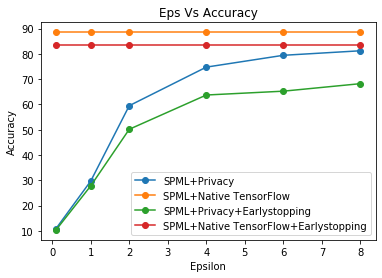
\includegraphics[width=\textwidth]{images/Training/MnistESAccuracy.png}
         \caption{Accuracy}
         \label{fig:EsMnistAccuracyTraining}
     \end{subfigure}
     \begin{subfigure}{0.5\textwidth}
         \includegraphics[width=\textwidth]{images/Training/MnistESLatency.png}
         \caption{Latency}
         \label{fig:EsMnistLatencyTraining}
     \end{subfigure}
        \caption{MNIST Dataset - Training - Earlystopping}
\end{figure}

As a continuation in the recent research, a distributed machine learning approach known as Federated learning \cite{86} is gaining lot of attention. In brief, it states that we don't need to share the sensitive and private data always instead we can just share the trained model. Then we can average out the model parameters of various trained model and in few rounds we will get good amount of accuracy without sharing the private and sensitive training data and hence data privacy can be preserved. We also explored this approach by running a small experiment on federated learning.

\subsection{Federated learning}
\label{sec:flTEE}
Till now we have seen the standard machine learning approaches wherein the training data is centralized and kept at one machine or data center. There are few issues with this approach such as if an attacker can breach the security of the data center then it may get hold of the whole training data. Another issue is that in small devices like mobile phones, the computation resources are limited therefore they cannot train the model on the whole training data. We need some way to decentralized the data and simultaneously reap the benefit of machine learning. This problem is solved by using Federated learning \cite{86}.

\begin{figure}[h!]
    \centering
    \includegraphics[width=10cm, height=10cm]{images/FL.pdf}
    \caption{Federated Learning}
    \label{fig:fld}
\end{figure}

Federated learning introduces a decentralized approach for machine learning. As show in Figure ~\ref{fig:fld}, in this approach, each device/user train the model with its local data and then send this trained local model to the server. The server aggregates the locally trained model from many devices to produce a final aggregate or global model. The server then sends the aggregate/global model for further training from each user's local data. In this way, the local data of the user is never shared, and only a trained local model and aggregate trained model is exchanged in every round of client-server communication. After a few rounds, the aggregate model will get good accuracy without even having actual training data and hence privacy of the user data is preserved as it is never shared.

\begin{table}[h!]
\begin{center}
\caption{Federated Learning Rounds - Accuracy in \%}
\label{tab:flrounds}
\begin{tabular}{|c|c|c|c|c|c|}
\hline
Rounds & Client1 & Client2 & Client3 & Client4 & Server \\
\hline
1      & 15.48   & 28.88   & 27.56   & 15.24   & 10.88  \\
\hline
2      & 33.96   & 31.28   & 21.52   & 22.16   & 27.2   \\
\hline
3      & 9       & 49.6    & 48.72   & 22.28   & 22.64  \\
\hline
4      & 72.48   & 58.92   & 77.68   & 66.28   & 69.72  \\
\hline
5      & 78.44   & 82.64   & 82.68   & 80.64   & 86.04  \\
\hline
6      & 89      & 85.68   & 89.8    & 89.2    & 89.8   \\
\hline
7      & 85.76   & 81.52   & 80.8    & 90.44   & 90.68  \\
\hline
8      & 92.04   & 89.04   & 90.56   & 91.52   & 92.4   \\
\hline
9      & 92.56   & 87.72   & 81.6    & 90.92   & 91.52  \\
\hline
10     & 92.28   & 92.64   & 93.36   & 92.48   & 93.48  \\
\hline
\end{tabular}
\end{center}
\end{table}

We tried this approach on the MNIST dataset \footnote{https://github.com/prbh695a/SPML/tree/master/Noise/MNIST/FL}. We split MNIST dataset into 4 parts, each part training 2500 samples. Then, we aggregated or averaged the model parameters of all these parts to produce an aggregate model. We call these parts as 'Client1', 'Client2', 'Client3' and 'Client4'. Clients are trained in native mode which can be on small individual devices (such as mobile phone), while aggregation is done on server using Intel SGX (hardware mode). 

We used test data of 2500 samples on the final aggregate model. As shown in table ~\ref{tab:flrounds}, in round-1 the aggregate model shows test accuracy of around 10.88\% and in round-10 the aggregate model started showing an accuracy of around 93.48\%. In this approach we simulated a scenario wherein we train the aggregate model in the SCONE hardware mode, while local training happened on each individual user's device (native mode) to reduce latency further.
